\documentclass[11pt]{article}

% Change "review" to "final" to generate the final (sometimes called camera-ready) version.
% Change to "preprint" to generate a non-anonymous version with page numbers.
\usepackage[review]{acl}

% Standard package includes
\usepackage{times}
\usepackage{latexsym}

% For proper rendering and hyphenation of words containing Latin characters (including in bib files)
\usepackage[T1]{fontenc}
% For Vietnamese characters
% \usepackage[T5]{fontenc}
% See https://www.latex-project.org/help/documentation/encguide.pdf for other character sets

% This assumes your files are encoded as UTF8
\usepackage[utf8]{inputenc}

% This is not strictly necessary, and may be commented out,
% but it will improve the layout of the manuscript,
% and will typically save some space.
\usepackage{microtype}

% This is also not strictly necessary, and may be commented out.
% However, it will improve the aesthetics of text in
% the typewriter font.
\usepackage{inconsolata}

%Including images in your LaTeX document requires adding
%additional package(s)
\usepackage{graphicx}

% TikZ for diagrams
\usepackage{tikz}
\usetikzlibrary{positioning, shapes, arrows}

% Better table formatting
\usepackage{booktabs}
\usepackage{xcolor}
\usepackage{array}
\usepackage{colortbl}
\usepackage{placeins}

% If the title and author information does not fit in the area allocated, uncomment the following
%
%\setlength\titlebox{<dim>}
%
% and set <dim> to something 5cm or larger.

\title{MOSAIC: Multi-Objective Search for Allocating Inference Cache Across LLM Decoder Layers}

\author{Anonymous}

%\author{
%  \textbf{First Author\textsuperscript{1}},
%  \textbf{Second Author\textsuperscript{1,2}},
%  \textbf{Third T. Author\textsuperscript{1}},
%  \textbf{Fourth Author\textsuperscript{1}},
%\\
%  \textbf{Fifth Author\textsuperscript{1,2}},
%  \textbf{Sixth Author\textsuperscript{1}},
%  \textbf{Seventh Author\textsuperscript{1}},
%  \textbf{Eighth Author \textsuperscript{1,2,3,4}},
%\\
%  \textbf{Ninth Author\textsuperscript{1}},
%  \textbf{Tenth Author\textsuperscript{1}},
%  \textbf{Eleventh E. Author\textsuperscript{1,2,3,4,5}},
%  \textbf{Twelfth Author\textsuperscript{1}},
%\\
%  \textbf{Thirteenth Author\textsuperscript{3}},
%  \textbf{Fourteenth F. Author\textsuperscript{2,4}},
%  \textbf{Fifteenth Author\textsuperscript{1}},
%  \textbf{Sixteenth Author\textsuperscript{1}},
%\\
%  \textbf{Seventeenth S. Author\textsuperscript{4,5}},
%  \textbf{Eighteenth Author\textsuperscript{3,4}},
%  \textbf{Nineteenth N. Author\textsuperscript{2,5}},
%  \textbf{Twentieth Author\textsuperscript{1}}
%\\
%\\
%  \textsuperscript{1}Affiliation 1,
%  \textsuperscript{2}Affiliation 2,
%  \textsuperscript{3}Affiliation 3,
%  \textsuperscript{4}Affiliation 4,
%  \textsuperscript{5}Affiliation 5
%\\
%  \small{
%    \textbf{Correspondence:} \href{mailto:email@domain}{email@domain}
%  }
%}

\begin{document}
\maketitle
\begin{abstract}
Key-Value (KV) cache consumption is a critical bottleneck for efficient LLM inference, especially on long-context workloads. While recent token eviction methods (SnapKV, H2O, AdaKV) reduce memory footprint, they apply uniform cache budgets across all transformer layers, overlooking the fact that different layers have fundamentally different token importance patterns. We propose MOSAIC, a multi-objective neural architecture search approach that discovers per-layer KV-cache budget allocations tailored to a given eviction algorithm. MOSAIC treats average cache budget and task score as competing objectives, runs a single unconstrained search to obtain a Pareto front of layer-wise allocations, selects a winner by full-data evaluation, and refines it with budget-constrained Bayesian optimization. On Llama-3-8B-Instruct with three eviction methods (SnapKV, H2O, AdaKV), MOSAIC beats uniform allocation in 38 of 42 evaluated (task, method, budget) cells, with gains of +3 to +33 points on RULER; the four losses are small ($\leq$0.74 points) and all on LongBench QA. A single search amortizes across budgets: the winner, proportionally rescaled with no further search, beats uniform in 46 of 55 cells. We further show that subsample-based search scores are unreliable on LongBench (the subsample's best candidate is the true best in only 7 of 29 cells), which makes full-data selection essential, and that the learned allocations consistently favor middle layers.
\end{abstract}

\section{Introduction}

\begin{figure*}[t]
  \centering
  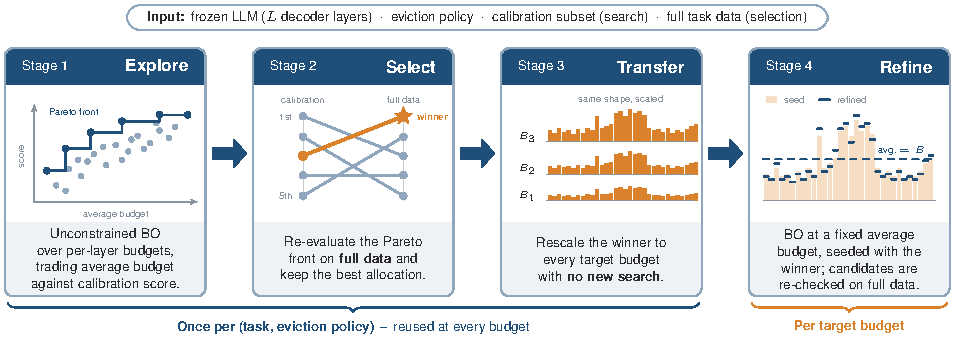
\includegraphics[width=\textwidth]{figures/figure1_pipeline.pdf}
  \caption{\textbf{The MOSAIC pipeline.} Stages 1--3 run once per (task, eviction policy): an unconstrained search on a calibration subset yields a Pareto front of per-layer allocations, full-data re-evaluation selects a winner, and the winner is proportionally rescaled to every target budget without further search. Stage 4 optionally refines each budget with constrained BO seeded by the rescaled winner. Bar profiles are schematic.}
  \label{fig:method}
\end{figure*}

The inference cost of large language models (LLMs) is increasingly dominated by attention memory consumption \citep{dao2022flashattention}. The key-value cache alone can consume 50–60\% of total memory on long-context workloads, becoming the primary bottleneck for throughput and latency scaling. Token eviction methods like H2O \citep{zhang2023h2o} and SnapKV \citep{li2024snapkv} address this by selectively dropping cache entries based on token importance, reducing memory by up to 90\% with minimal accuracy loss. However, these methods apply the same memory budget to every transformer layer. Layer-wise allocation schemes exist, but they either fix the shape of the allocation in advance \citep{cai2024pyramidkv}, derive it from attention statistics \citep{qin2025cake}, or search coarse layer groups separately for each target budget \citep{yu2025evolkv}. This overlooks a critical insight: different layers prioritize tokens differently. In retrieval-heavy tasks, lower layers retrieve surface-level information while higher layers perform reasoning; allocating uniform cache across all layers wastes memory on less-critical layers while starving critical ones.

This paper introduces MOSAIC, a method that automatically optimizes per-layer KV-cache budgets under a target memory constraint using multi-objective neural architecture search. Rather than hand-tuning layer-specific heuristics or using coarse grouped allocation (4–8 groups), MOSAIC directly searches the 32-dimensional per-layer budget space using Bayesian optimization guided by a surrogate MLP. We evaluate MOSAIC across three eviction methods (SnapKV, H2O, AdaKV) and two benchmarks: LongBench (4 task categories) and RULER (11 in-context retrieval subtasks). On RULER, where layer importance is most pronounced, per-layer optimization yields large gains (+3.1 to +33.3 points over uniform) while maintaining strict memory budgets, concentrated on the hardest needle-retrieval subtasks. On LongBench, gains are smaller: every CODE cell improves, while QA shows four small losses that we report explicitly.

Our contributions are: (i) a four-stage search pipeline in which one unconstrained search transfers across budgets (the rescaled winner beats uniform in 46/55 cells), so the search cost is amortized rather than paid per budget; (ii) evidence that calibration-subsample scores do not reliably rank configurations on LongBench, motivating full-data selection and showing that Bayesian refinement can over-fit a noisy search signal; and (iii) an analysis of the learned allocations, which consistently give middle layers (L10, L14–L20) more than their uniform share.

\section{Related Work}

\subsection{KV-Cache Optimization}

\textbf{Token eviction.} Eviction methods reduce KV-cache memory by retaining only the tokens judged important. H2O \citep{zhang2023h2o} keeps ``heavy hitters'', tokens with high accumulated attention, together with a window of recent tokens. SnapKV \citep{li2024snapkv} selects, for each attention head, the prompt positions that receive the most attention from an observation window at the end of the prompt. Both give every layer the same budget.

\textbf{Budget allocation.} A second line of work redistributes a fixed total budget instead of changing how tokens are scored. Ada-KV \citep{feng2024adakv} allocates budget adaptively across the heads of a layer. PyramidKV \citep{cai2024pyramidkv} assigns layer budgets following a fixed pyramidal shape, larger in lower layers and smaller in higher ones. CAKE \citep{qin2025cake} derives per-layer budgets from layer preferences measured on attention patterns. Closest to our work, EvolKV \citep{yu2025evolkv} treats per-layer budgets as optimization variables, partitions layers into groups, and runs evolutionary search against downstream task score, repeating the search for each target budget. MOSAIC differs in three ways: it searches all 32 layer budgets without grouping; a single unconstrained search yields a winner that transfers across budgets; and it selects configurations on full data, which we show is necessary because subsample scores do not reliably rank configurations on LongBench.

\subsection{Neural Architecture Search}

NAS has been successfully applied to model compression, hardware optimization, and neural network design \citep{elsken2018neural}. Multi-objective NAS balances competing goals (e.g., accuracy vs. latency) using Pareto-front optimization. MOSAIC adapts this machinery to the KV-cache allocation problem, treating per-layer budget as an architecture parameter.

\section{Method}

\subsection{Problem Formulation}

Given an eviction method $M$ and target budget $B$ (average tokens per layer), we seek to find a vector $\mathbf{b} = (b_1, \ldots, b_{32}) \in [b_{\min}, b_{\max}]^{32}$ that maximizes task performance while maintaining $\frac{1}{32}\sum_{i=1}^{32} b_i = B$. This is a 32-dimensional constrained optimization problem. We use a per-layer floor $b_{\min} = 64$: SnapKV and H2O always retain a fixed 8-token recent window, so a layer at budget 16 would select only 8 tokens by attention, a degenerate regime that an earlier floor of 16 let the search exploit (up to 66\% of layers parked at the floor). Each configuration is encoded as $\mathbf{x} \in [0,1]^{32}$. The unconstrained search is multi-objective: it minimizes the mean per-layer budget $f_1(\mathbf{b}) = \frac{1}{32}\sum_i b_i$ and maximizes the task score $f_2(\mathbf{b})$ on a calibration subsample. The budget-constrained variant (Stage 4) instead fixes $f_1 = B$ by rescaling the per-layer weights so that their mean equals $B$ exactly.

\textbf{Search step.} All stages share one classifier-guided Bayesian optimization procedure. After each evaluation, the archive is non-dominated sorted, an MLP classifier (two hidden layers of 32 units) is trained to separate the rank-1 configurations from the rest, and differential evolution maximizes the classifier's probability of rank 1 over $[0,1]^{32}$ to propose the next configuration, one evaluation per iteration. We call these proposals BO proposals. The evaluation cap is 1000; in practice runs were stopped once the archive had settled.

\subsection{Search Procedure (MOSAIC — Four-Stage Pipeline)}

The search is divided into four distinct stages:

\textbf{Stage 1 (Unconstrained Multi-Budget NAS):} Search a discrete per-layer grid, $\{64,128,256,512,1024\}$ on LongBench and seven levels from 64 to 4096 on RULER, with no budget constraint. The initial design has 64 points: the uniform allocation at every grid level (5 on LongBench, 7 on RULER) plus Latin Hypercube samples (59 and 57). Guided iterations then trace out the budget--score Pareto front.

\textbf{Stage 2 (Winner Selection via Full-Data Eval):} Re-evaluate every configuration on the Stage 1 Pareto front (13--17 configurations per category for AdaKV) on the full test data, and keep the \textbf{winner shape}: the shaped configuration with the highest full-data score. This winner becomes a universal anchor for all subsequent budget-constrained searches. Full-data selection is essential rather than a formality. On LongBench, search-time calibration scores are optimistic (by 5.7 points for SnapKV and H2O, and 1.1 for AdaKV, whose LongBench searches used a 30\% instead of a 10\% subsample) and rank candidates poorly: the calibration-best candidate is the true full-data best in only 5 of 20 SnapKV/H2O cells and 2 of 9 AdaKV cells (mean Kendall $\tau \approx 0$ and $0.47$). On RULER, calibration is faithful for all three methods ($\tau = 0.77$--$1.00$; 12 of 13 correct picks). Table~\ref{tab:calib} summarizes this; per-cell values are in Appendix~\ref{app:calib}.

\begin{table}[htbp]
  \centering
  \footnotesize
  \setlength{\tabcolsep}{2.5pt}
  \begin{tabular}{@{} l l r r r r r @{}}
    \toprule
    \textbf{Bench.} & \textbf{Method} & \textbf{Cells} & \textbf{Gap} & \textbf{$\tau$} & \textbf{Picks} & \textbf{Regret} \\
    \midrule
    \rowcolor{gray!10}
    LongBench & H2O    & 8  & $+5.84$ & $-0.10$ & 1/8  & 0.99 \\
    LongBench & SnapKV & 12 & $+5.65$ & $+0.07$ & 4/12 & 0.62 \\
    \rowcolor{gray!10}
    RULER     & H2O    & 4  & $+0.09$ & $+0.82$ & 4/4  & 0.00 \\
    RULER     & SnapKV & 3  & $-0.13$ & $+1.00$ & 3/3  & 0.00 \\
    \midrule
    \rowcolor{gray!10}
    LongBench & AdaKV$^\ast$ & 9 & $+1.14$ & $+0.47$ & 2/9 & 0.40 \\
    RULER     & AdaKV  & 6  & $-0.20$ & $+0.77$ & 5/6  & 0.02 \\
    \bottomrule
  \end{tabular}
  \caption{\textbf{Calibration vs.\ full-data scores.} Gap: mean calibration minus full-data score. $\tau$: mean Kendall correlation between the two rankings of each cell's five candidates. Picks: cells where the calibration-best candidate is also full-data best. Regret: mean full-data points lost by trusting calibration. Calibration subsample 10\%, except $^\ast$30\%.}
  \label{tab:calib}
\end{table}

\textbf{Stage 3 (Winner Rescaling to Fixed Budgets):} Take the winner shape discovered in Stage 2 and rescale it to match fixed target budgets $B \in \{64, 128, 256, 512, 1024, 2048\}$. Evaluate each rescaled configuration on full test data. These Stage 3 results (\textbf{Winner-Rescaled}) require no further search, and they already beat uniform in 46 of 55 (category, method, budget) cells, including shapes found at an average budget of $\sim$2400 transferred down to 128. By contrast, EvolKV must re-run its full search for every budget. Table~\ref{tab:transfer} summarizes the transfer; all 55 cells are in Appendix~\ref{app:transfer}, and search costs in Appendix~\ref{app:cost}.

\begin{table}[htbp]
  \centering
  \footnotesize
  \setlength{\tabcolsep}{2.5pt}
  \begin{tabular}{@{} l l r r r @{}}
    \toprule
    \textbf{Category} & \textbf{Method} & \textbf{Natural} & \textbf{Wins} & \textbf{Mean $\Delta$} \\
    \midrule
    \rowcolor{gray!10}
    Code      & H2O    & 2456 & 3/4 & $+0.54$ \\
    Code      & SnapKV & 430  & 4/4 & $+1.66$ \\
    \rowcolor{gray!10}
    MultiDoc  & H2O    & 448  & 3/4 & $+0.55$ \\
    MultiDoc  & SnapKV & 274  & 3/4 & $+0.32$ \\
    \rowcolor{gray!10}
    SingleDoc & H2O    & 518  & 2/3 & $+0.69$ \\
    SingleDoc & SnapKV & 506  & 3/4 & $+0.04$ \\
    \rowcolor{gray!10}
    Summ      & H2O    & 552  & 3/3 & $+0.10$ \\
    Summ      & SnapKV & 732  & 3/3 & $+0.17$ \\
    \rowcolor{gray!10}
    RULER     & H2O    & 2180 & 2/3 & $+8.70$ \\
    RULER     & SnapKV & 1756 & 7/7 & $+6.99$ \\
    \midrule
    \rowcolor{gray!10}
    Code      & AdaKV  & 482  & 2/3 & $+0.38$ \\
    MultiDoc  & AdaKV  & 188  & 2/3 & $+0.22$ \\
    \rowcolor{gray!10}
    SingleDoc & AdaKV  & 464  & 2/3 & $+0.12$ \\
    RULER     & AdaKV  & 2536 & 7/7 & $+2.16$ \\
    \midrule
    \multicolumn{3}{@{}l}{\textbf{Total}} & \textbf{46/55} & \\
    \bottomrule
  \end{tabular}
  \caption{\textbf{One search, many budgets.} The Stage 2 winner, found once at its natural average budget, is rescaled to every target budget with no further search. Wins: budgets where it beats uniform on full data.}
  \label{tab:transfer}
\end{table}

\textbf{Stage 4 (Budget-Constrained Adaptive Search):} For each target budget $B$, perform a dedicated BO search constrained to produce configurations with average budget exactly $B$. Seed this search with: (i) the Stage 2 winner rescaled to budget $B$ (from Stage 3), (ii) six heuristic shapes (uniform, ascending and descending ramps, middle- and edge-heavy triangles, and an alternating low/high pattern), and (iii) 57 Latin Hypercube (LHS) seed points, all drawn inside the constrained per-layer space (continuous weights rescaled to mean $B$). Guided BO iterations then extend this pool; run lengths varied from 97 to 1000 evaluations across methods and cells. The pool (rescaled winner, heuristic shapes, LHS seed points and BO proposals) is MOSAIC's candidate set for that budget: the best calibration-scored candidate of each type is re-evaluated on full data together with uniform, and \textbf{MOSAIC's final configuration is the best of these on full data}. Which candidate type wins is analysed in Section~\ref{sec:which-stage}.


\section{Experiments}

\begin{table*}[t]
  \centering
  \small
  \setlength{\tabcolsep}{12pt}
  \begin{tabular}{@{} l l r r r @{}}
    \toprule
    \textbf{Category} & \textbf{Method} & \textbf{Uniform-512} & \textbf{Best NAS} & \textbf{NAS Cost} \\
    \midrule
    \rowcolor{gray!10}
    CODE & SnapKV & 56.73 & \textbf{58.26} (+1.53) & 430 (84\%) \\
    CODE & H2O & 52.81 & 53.45 (+0.64) & 398 (78\%) \\
    \rowcolor{gray!10}
    CODE & AdaKV & 58.70 & 60.55 (+1.85) & 396 (77\%) \\
    MULTI\_DOC\_QA & SnapKV & 35.77 & \textbf{36.14} (+0.37) & 274 (54\%) \\
    \rowcolor{gray!10}
    MULTI\_DOC\_QA & H2O & 32.98 & \textbf{33.59} (+0.61) & 364 (71\%) \\
    SINGLE\_DOC\_QA & SnapKV & 35.97 & 36.33 (+0.36) & 506 (99\%) \\
    \rowcolor{gray!10}
    SUMMARIZATION & SnapKV & 23.44 & 23.54 (+0.10) & 510 (100\%) \\
    \bottomrule
  \end{tabular}
  \caption{\textbf{Stage 2 Pareto configurations vs.\ uniform-512 (LongBench, full data).} Each row is a configuration from the Stage 2 Pareto front with average budget at most 512; ``NAS Cost'' is its average budget and its fraction of 512. Parentheses: gain over uniform-512. Bold: also beats uniform at every budget up to 1024 (not available for AdaKV, whose uniform runs stop at 512). Same-budget comparisons are in Appendix~\ref{app:cells}.}
  \label{tab:longbench-summary}
\end{table*}

\begin{table*}[t]
  \centering
  \small
  \setlength{\tabcolsep}{16pt}
  \begin{tabular}{@{} l r r r @{}}
    \toprule
    \textbf{Budget} & \textbf{Uniform} & \textbf{MOSAIC} & \textbf{Gain (pts)} \\
    \midrule
    \multicolumn{4}{c}{\textbf{\textit{SnapKV}}} \\
    \midrule
    \rowcolor{gray!10}
    64 & 34.64 & 44.99$^\dagger$ & +10.35 \\
    128 & 51.56 & 61.08$^\dagger$ & +9.52 \\
    \rowcolor{gray!10}
    256 & 68.06 & 72.49$^\dagger$ & +4.43 \\
    512 & 78.62 & 81.76$^\dagger$ & +3.14 \\
    \rowcolor{gray!10}
    1024 & 85.67 & 93.80 & +8.13 \\
    1536 & 88.62 & 98.35 & +9.73 \\
    \rowcolor{gray!10}
    2048 & 92.93 & 98.91 & +5.98 \\
    \midrule
    \multicolumn{4}{c}{\textbf{\textit{H2O}}} \\
    \midrule
    \rowcolor{gray!10}
    128 & 12.19 & 15.39 & +3.19 \\
    1024 & 44.35 & 62.52 & +18.17 \\
    \rowcolor{gray!10}
    1536 & 53.39 & 86.05 & +32.66 \\
    2048 & 62.82 & 96.14 & +33.32 \\
    \midrule
    \multicolumn{4}{c}{\textbf{\textit{AdaKV}}} \\
    \midrule
    \rowcolor{gray!10}
    64 & 35.81 & 35.97$^\dagger$ & +0.16 \\
    128 & 50.87 & 57.40 & +6.53 \\
    \rowcolor{gray!10}
    256 & 68.02 & 72.10 & +4.08 \\
    512 & 78.22 & 83.08 & +4.85 \\
    \rowcolor{gray!10}
    1024 & 86.87 & 93.78 & +6.91 \\
    1536 & 89.75 & 97.99 & +8.25 \\
    \rowcolor{gray!10}
    2048 & 93.90 & 98.65 & +4.75 \\
    \bottomrule
  \end{tabular}
  \caption{\textbf{RULER results (full data, string-match accuracy averaged over 11 subtasks).} Uniform allocation vs.\ MOSAIC's final configuration at the same average budget, i.e.\ the best full-data candidate in its pool (rescaled winner, heuristic shapes, LHS seed points, BO proposals). $^\dagger$No Stage 4 search at this budget: rescaled Stage 3 winner only. Which candidate type wins in each cell is analysed in Table~\ref{tab:stage-best} and listed in Appendix~\ref{app:cells}. Floor 16 applies at B1024--B2048 for all methods, at B64--B512 for SnapKV, and at B64 for AdaKV (see Caveat).}
  \label{tab:ruler-summary}
\end{table*}


\subsection{Setup}

\textbf{Model:} Meta-Llama-3-8B-Instruct. \textbf{Benchmarks:} LongBench (4 categories, 11 datasets) and RULER (11 in-context retrieval subtasks). \textbf{Methods:} SnapKV, H2O, AdaKV. \textbf{Budgets:} 64–2048 average tokens per layer. \textbf{Search signal:} a 10\% calibration subsample, except 30\% for AdaKV on LongBench; all reported scores are full-data. AdaKV Summarization is still running and is not reported. All experiments run on A100 GPUs; LongBench uses full dataset ($\geq 100$ samples per dataset); RULER uses all 500 samples per task.

\begin{figure*}[t]
  \centering
  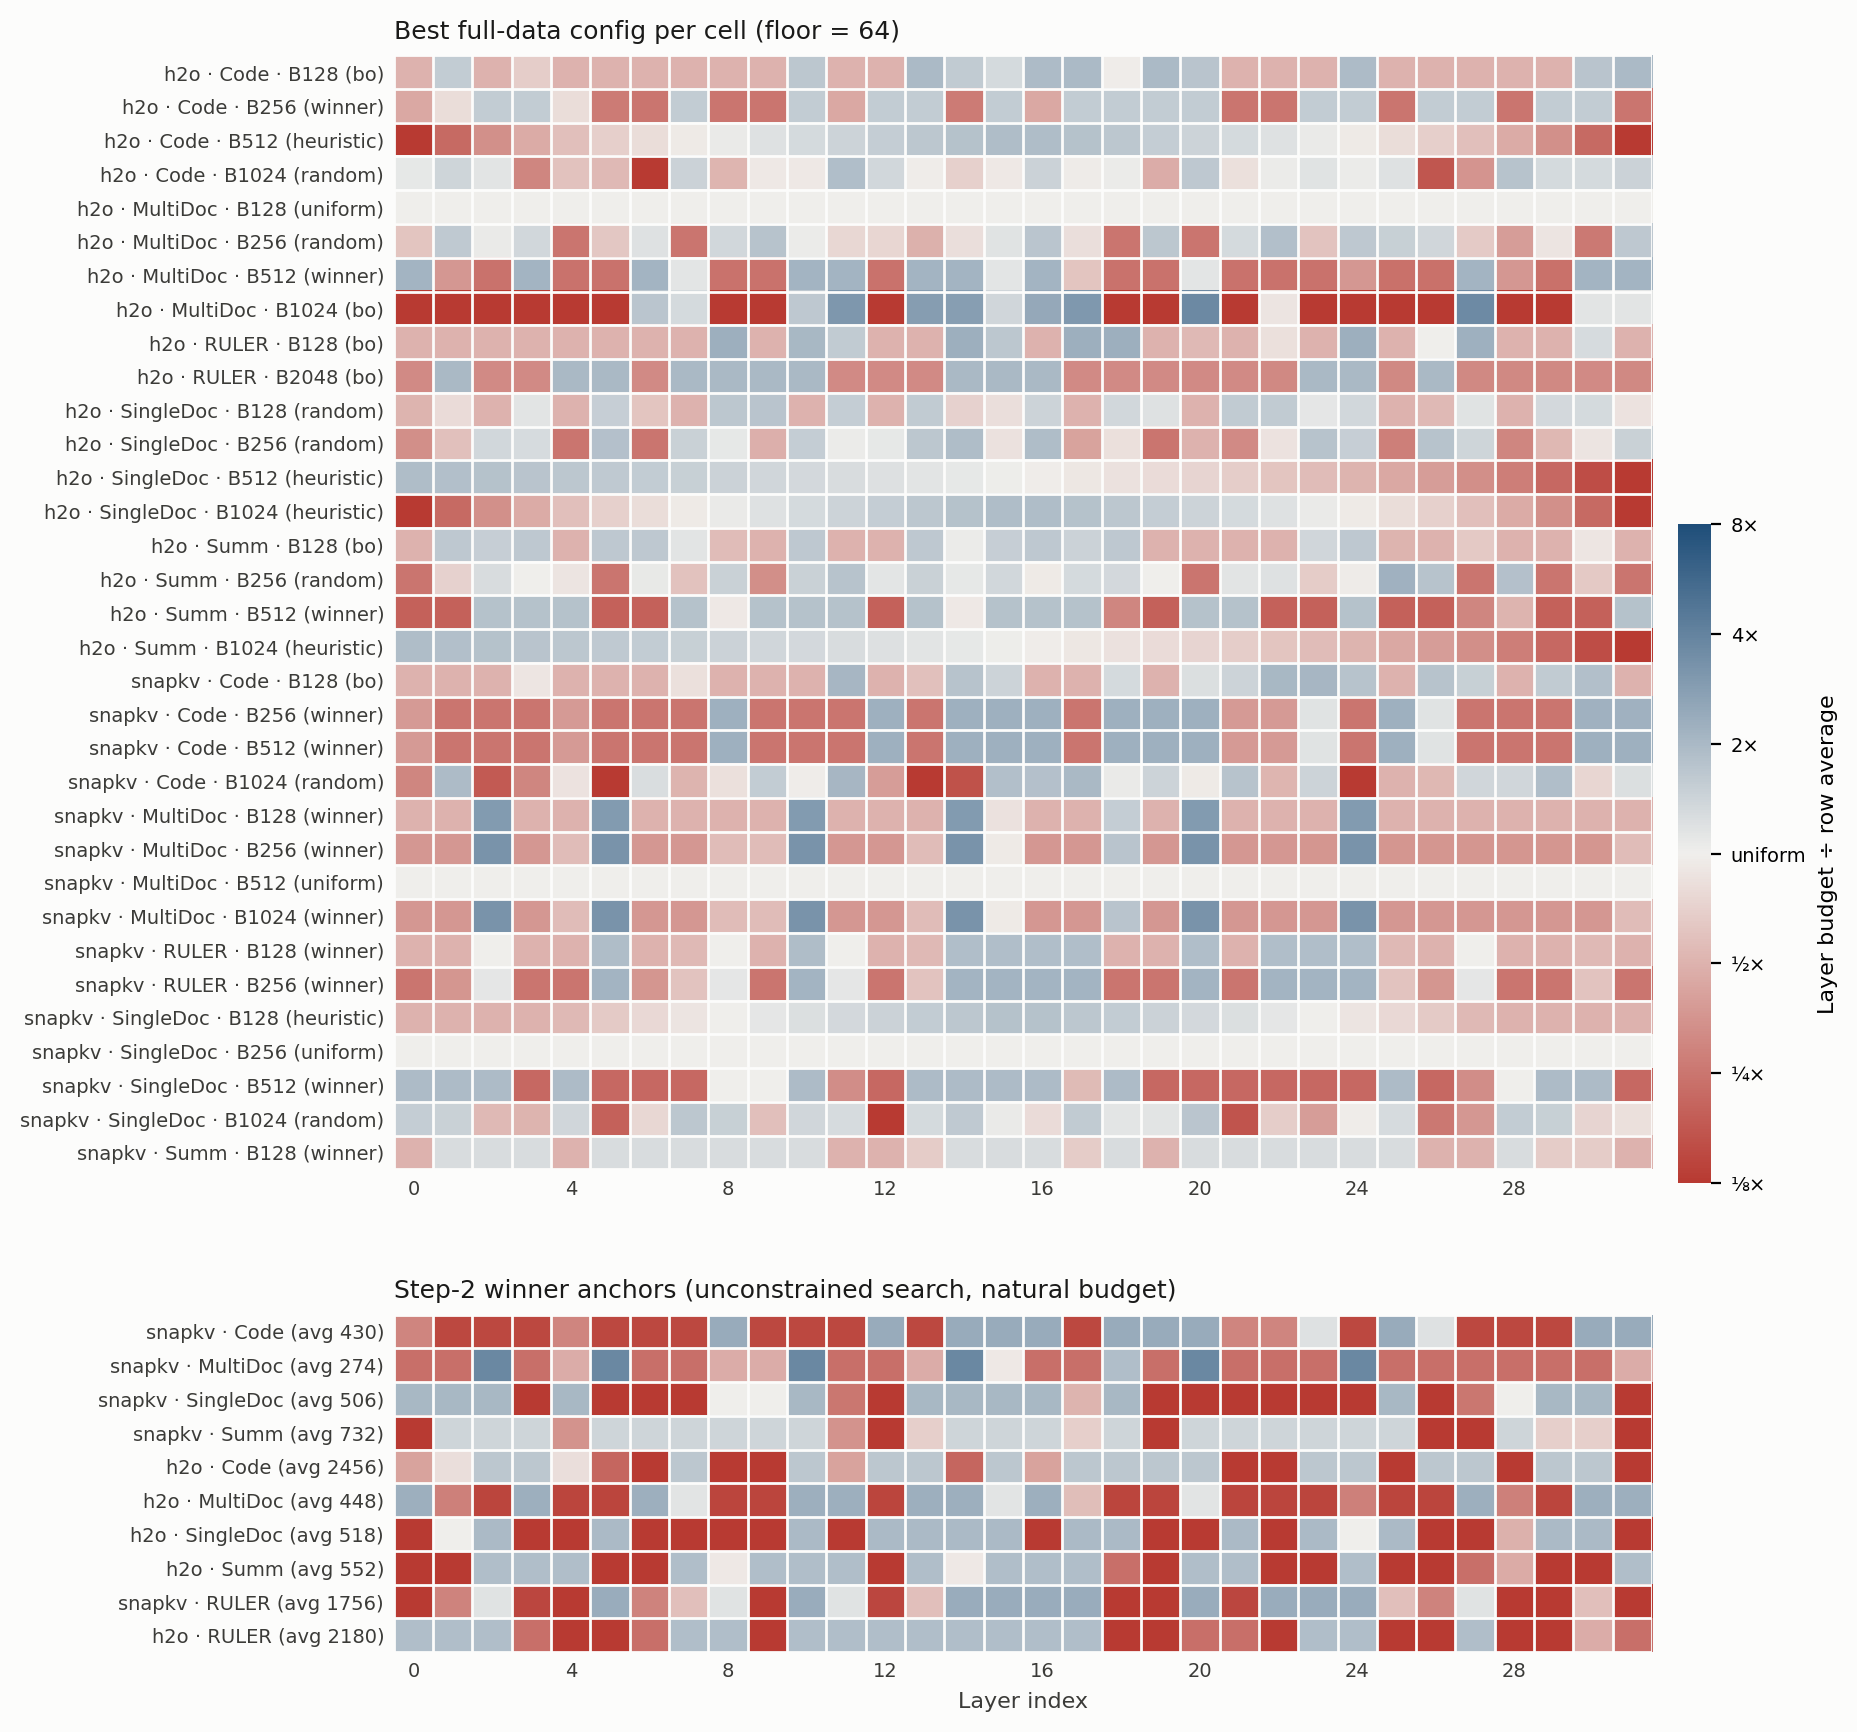
\includegraphics[width=0.8\textwidth]{figures/A4_layer_importance_heatmap.png}
  \caption{\textbf{Learned per-layer allocations (floor = 64).} Colour shows each layer's budget divided by the row average on a log$_2$ scale (blue: more than the uniform share; red: less). \textit{Top:} best full-data configuration per (method, category, budget) cell for SnapKV and H2O on LongBench and RULER B128; the candidate type that produced it is shown in parentheses (``random'' denotes an LHS seed point). \textit{Bottom:} Stage 2 winner anchors from the unconstrained search, at their natural average budget. Middle layers (L10, L14--L20) receive more than their uniform share in 58--74\% of allocations, while early (L0--L9) and late (L21--L29) layers are mostly under-allocated (13--35\%).}
  \label{fig:heatmap}
\end{figure*}

\subsection{Key Findings — LongBench}
\label{sec:which-stage}

Table~\ref{tab:longbench-summary} asks a cost question: for each category and method, a configuration from the Stage 2 Pareto front with average budget at most 512, evaluated on full data, is compared with uniform allocation at 512. Same-budget comparisons are in Table~\ref{tab:stage-best} and Appendix~\ref{app:cells}. The clearest savings are on CODE and MULTI\_DOC\_QA:

\begin{itemize}
\item \textbf{CODE:} SnapKV's configuration (58.26 at average budget 430, 84\% of 512) beats uniform at every budget up to 1024 (max 56.73); AdaKV's (60.55 at 396) beats uniform-512 (58.70).
\item \textbf{MULTI\_DOC\_QA:} SnapKV's configuration (36.14 at 274) beats uniform-1024 (35.87) at 27\% of its cache.
\item \textbf{SINGLE\_DOC\_QA \& SUMMARIZATION:} Gains are modest ($\leq$ 1 point).
\end{itemize}

\textbf{Where NAS loses.} Across all evaluated cells, NAS beats uniform in 38 of 42 (SnapKV and H2O: 24/27; AdaKV: 14/15), including every CODE and RULER cell. The four losses are all LongBench QA and small: H2O MULTI\_DOC\_QA at B128 ($-0.41$), SnapKV MULTI\_DOC\_QA at B512 ($-0.04$), SnapKV SINGLE\_DOC\_QA at B256 ($-0.74$), and AdaKV SINGLE\_DOC\_QA at B512 ($-0.20$).

\textbf{Which stage matters.} For SnapKV and H2O on LongBench, the rescaled Stage 3 winner is the most reliable configuration (best in 8 of 20 cells, median $+0.63$ over uniform), while the Stage 4 BO optimum is on average slightly \emph{worse} than uniform (median $-0.38$), consistent with BO over-fitting the noisy 10\% calibration signal described in Stage 2. In 4 of these 20 cells the best full-data configuration is one of the Latin Hypercube seed points rather than a BO proposal (Table~\ref{tab:stage-best}, Figure~\ref{fig:heatmap}). These points are still drawn from MOSAIC's constrained per-layer space (floor 64, fixed average budget) and reach the final comparison only through full-data selection among the top calibration candidates.

AdaKV behaves differently on LongBench: its BO optimum is above uniform (median $+0.62$) while its rescaled winner is weaker (median $+0.33$). This does not mean its search signal is reliable. Even with a 30\% subsample, the calibration pick is the true best in only 2 of 9 AdaKV LongBench cells, and BO's calibration gain over uniform overstates its full-data gain in all 9 cells, by 1.44 points on average; BO stays ahead of uniform, but by much less than the search score suggests. On RULER, where calibration is faithful for all three methods, no single stage dominates: BO is best in 5 of 7 SnapKV/H2O cells, but LHS seed points are best in 4 of 6 AdaKV cells. The winning AdaKV seed is the same point of the fixed Latin Hypercube design in all four of those cells, decoded at each budget, so it acts as a second shape that transfers across budgets. What holds across all three methods is that some non-uniform per-layer allocation beats uniform in every RULER cell. We therefore attribute MOSAIC's gains to the per-layer search space, full-data selection, and cross-budget transfer. Stage 4 BO helps in some settings but is not reliably better than its own seed points, and a random-search baseline at equal evaluation budget remains to be run. Per-cell results for all 42 cells are in Appendix~\ref{app:cells}.

\begin{table}[htbp]
  \centering
  \footnotesize
  \setlength{\tabcolsep}{2.5pt}
  \begin{tabular}{@{} l r r r r r r @{}}
    \toprule
    & \multicolumn{3}{c}{\textbf{LongBench}} & \multicolumn{3}{c}{\textbf{RULER}} \\
    \cmidrule(lr){2-4} \cmidrule(lr){5-7}
    \textbf{Stage} & \#best & mean & med. & \#best & mean & med. \\
    \midrule
    \multicolumn{7}{@{}l}{\textit{SnapKV + H2O} (20 LongBench / 7 RULER cells)} \\
    Uniform   & 3 & -- & -- & 0 & -- & -- \\
    Heuristic & 2 & $+0.26$ & $+0.17$ & 0 & $+14.79$ & $+29.69$ \\
    \rowcolor{gray!10}
    Winner    & \textbf{8} & $\mathbf{+0.62}$ & $\mathbf{+0.63}$ & 2 & $+7.93$ & $+9.07$ \\
    LHS seed  & 4 & $+0.20$ & $+0.27$ & 0 & $+10.34$ & $+8.24$ \\
    \rowcolor{gray!10}
    BO        & 3 & $-0.24$ & $-0.38$ & \textbf{5} & $\mathbf{+19.10}$ & $\mathbf{+18.17}$ \\
    \midrule
    \multicolumn{7}{@{}l}{\textit{AdaKV} (9 LongBench / 6 RULER cells)} \\
    Uniform   & 1 & -- & -- & 0 & -- & -- \\
    Heuristic & \textbf{3} & $+0.63$ & $\mathbf{+0.90}$ & 1 & $+3.69$ & $+3.22$ \\
    \rowcolor{gray!10}
    Winner    & 1 & $+0.24$ & $+0.33$ & 0 & $+2.50$ & $+2.50$ \\
    LHS seed  & 1 & $\mathbf{+0.64}$ & $+0.38$ & \textbf{4} & $\mathbf{+5.27}$ & $\mathbf{+4.75}$ \\
    \rowcolor{gray!10}
    BO        & \textbf{3} & $+0.56$ & $+0.62$ & 1 & $+3.93$ & $+4.16$ \\
    \bottomrule
  \end{tabular}
  \caption{\textbf{Which stage produces the best configuration.} Candidates are the members of MOSAIC's Stage 3/4 pool (LHS seed: best Latin Hypercube seed point). \#best: cells where that candidate has the highest full-data score. Mean/median: full-data gain over uniform across all cells where the candidate was evaluated. The best stage depends on the method and benchmark; for SnapKV and H2O on LongBench, BO over-fits and the rescaled winner is most reliable.}
  \label{tab:stage-best}
\end{table}


\subsection{Key Findings — RULER}

RULER's needle-in-haystack tasks show much larger gains from per-layer optimization. Table~\ref{tab:ruler-summary} gives, for each method and budget, MOSAIC's final configuration: the best candidate in its pool on full data. For SnapKV at B64--B512 and AdaKV at B64, no Stage 4 search was run, so the entry is the rescaled Stage 3 winner. Every RULER cell improves on uniform, for all three methods:

\begin{itemize}
\item \textbf{SnapKV:} $+3.1$ to $+10.4$; at B1024 MOSAIC reaches 93.80 against 85.67 for uniform.
\item \textbf{H2O:} the largest gains, $+18.2$ to $+33.3$ at B1024--B2048; at B128 (floor 64) the gain is $+3.2$.
\item \textbf{AdaKV:} $+4.1$ to $+8.3$ from B128 to B2048.
\end{itemize}

These gains are substantially larger than on LongBench, reflecting RULER's structural task design: correct answers sit in specific positional windows. The gains concentrate on the hardest needle subtasks, where uniform allocation nearly fails. For SnapKV and H2O (floor-clean cells), NAS adds $+44.6$ on niah\_multikey\_3 and $+37.4$ on niah\_single\_3, versus $-0.6$, $+2.7$ and $+3.6$ on CWE, FWE and VT; for AdaKV the largest gains are also on niah\_multikey\_3 ($+49$ to $+82$ at B1024--B2048; Appendix~\ref{app:ruler}).

\textbf{Caveat.} The RULER B1024 cells of all three methods were searched under the earlier per-layer floor of 16; SnapKV and H2O use it (31\% and 66\% of layers sit at 16), and the floor-16 H2O B1024 configuration trades CWE accuracy (98$\rightarrow$22) for needle retrieval. B1536 and B2048 also ran with floor 16; for SnapKV and H2O their best configurations never reach it, while one AdaKV B1536 candidate (not the final configuration) does. AdaKV B64 also used floor 16.




\section{Analysis}

% Figure 4 (task gains) disabled until regenerated from per-cell data (PAPER_ISSUES.md item 10):
% \begin{figure}[t]
%   \centering
%   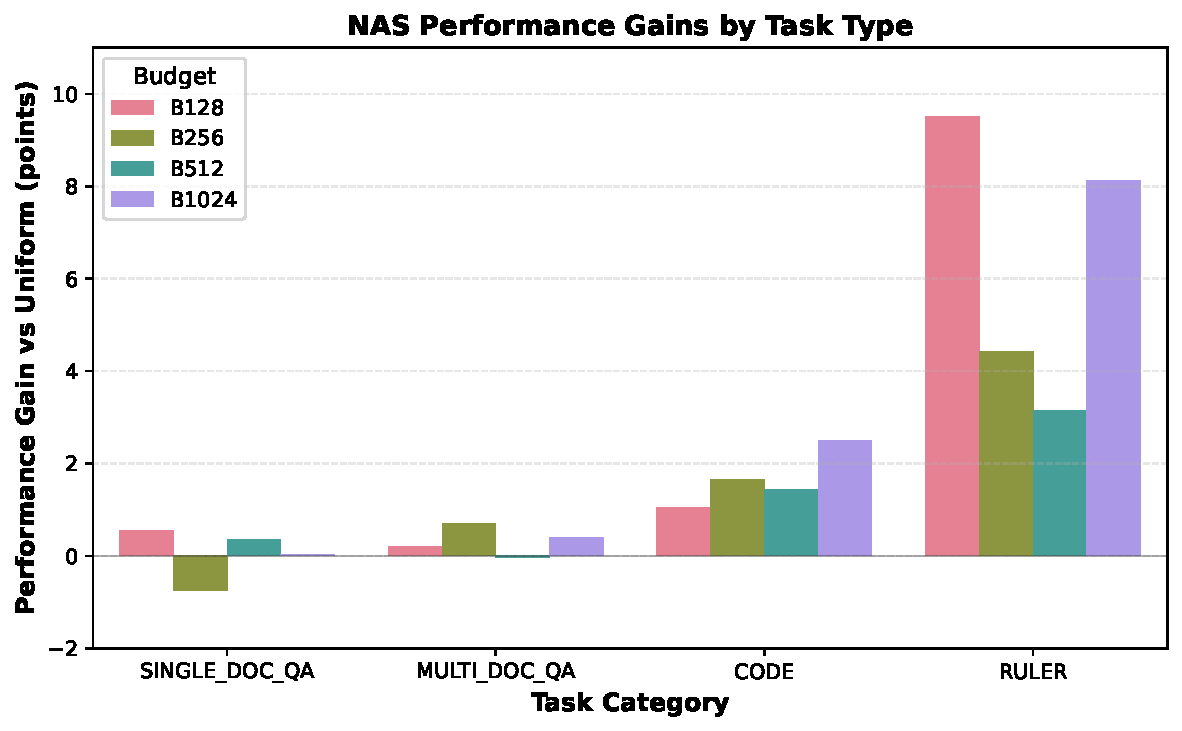
\includegraphics[width=0.95\columnwidth]{figures/figure4_task_gains.pdf}
%   \caption{Performance gains of NAS best configuration over uniform allocation, by task category and budget. RULER (needle-in-haystack retrieval) shows dramatic gains (+4 to +10 points across budgets), while LongBench QA tasks show modest gains ($\leq$ 1 point). CODE tasks exhibit intermediate gains (+1 to +2.5 points). This pattern reflects task structure: RULER's positional importance is highly layer-dependent, enabling NAS to achieve substantial improvements through selective reallocation. LongBench QA distributes evidence more evenly across context, leaving less room for per-layer optimization to help.}
%   \label{fig:gains}
% \end{figure}


\subsection{Why Task Type Matters}

LongBench QA tasks (SINGLE\_DOC\_QA, MULTI\_DOC\_QA) treat all layers nearly equally because evidence is scattered across the context. RULER's needle-in-haystack design forces lower layers to retrieve surface tokens early and higher layers to reason; this structure gives NAS crisp layer-importance signals to optimize. Code completion exhibits intermediate behavior: function signatures and recent edits sit at predictable positions, more structured than QA but less strictly needle-like than RULER.

\subsection{Shared Layer Structure}

Although each cell is searched independently, the resulting allocations share a common shape (Figure~\ref{fig:heatmap}). Across categories, budgets and the two methods analysed (SnapKV and H2O), middle layers (L10, L14--L20) receive more than their uniform share in 58--74\% of allocations, whereas early (L0--L9) and late (L21--L29) layers are mostly starved (13--35\%). This structure is consistent with the rescaled Stage 3 winner transferring well across budgets.

\subsection{Method-Specific Patterns}

H2O shows the largest absolute RULER gains (+18–33 points) because its unconstrained-search winner often overallocates to specific layers that become underfunded at low budgets; reallocation recovers this. SnapKV's gains are more modest because its simpler scoring already adapts reasonably per layer. AdaKV, which already allocates budget adaptively across heads within a layer, still gains from reallocation across layers: $+4.1$ to $+8.3$ on RULER and up to $+1.98$ on LongBench, comparable to SnapKV.

\section{Ablation: Grouped-CMA-ES}

We compare MOSAIC's full 32-layer search against a grouped-CMA-ES baseline inspired by EvolKV \citep{yu2025evolkv}, which partitions the 32 layers into 4 groups of 8 and optimizes each group independently with real CMA-ES. Evaluated on SnapKV CODE and SINGLE\_DOC\_QA at budgets 128/512/1024:

\begin{table}[t]
  \centering
  \small
  \setlength{\tabcolsep}{8pt}
  \begin{tabular}{@{} l c r r @{}}
    \toprule
    \textbf{Task} & \textbf{B} & \textbf{Grouped}$^*$ & \textbf{MOSAIC} \\
    \midrule
    \rowcolor{gray!10}
    CODE & 128 & 63.80 & 56.10 \\
    CODE & 512 & 65.30 & 58.17 \\
    \rowcolor{gray!10}
    CODE & 1024 & 66.34 & 58.91 \\
    SINGLE\_DOC & 128 & 43.31 & 33.67 \\
    \rowcolor{gray!10}
    SINGLE\_DOC & 512 & 43.67 & 36.33 \\
    SINGLE\_DOC & 1024 & 43.09 & 37.01 \\
    \bottomrule
  \end{tabular}
  \caption{\textbf{Ablation: Grouped-CMA-ES vs. Full Per-Layer NAS.} $^*$Grouped-CMA-ES (EvolKV-style): 4 groups of 8 layers, scored on calibration subsamples. MOSAIC: full 32 layers, scored on full test data. Not directly comparable (full-data re-evaluation of the grouped baseline is pending); included for directional reference only.}
  \label{tab:ablation}
\end{table}

The grouped baseline's higher numbers are calibration-subsample scores, which on LongBench exceed full-data scores by 5.7 points on average (Stage 2), so they should not be read as a win over full per-layer search. Full-data re-evaluation of the grouped baseline is pending. Search cost is comparable, not lower: on the 6 matched cells, with the same A100 hardware and harness, EvolKV-style search costs 53.7 GPU-hours versus 51.1 for our Stage 4 at the 200-evaluation cap (EvolKV: 600 evaluations $\times$ 30 samples; ours: $\sim$200 $\times$ 55--100 samples). MOSAIC's efficiency advantage is amortization: one Stage 1 search serves every budget.

\section{Limitations}

\begin{enumerate}
\item \textbf{Search cost:} cost depends strongly on the eviction method. A SnapKV Stage 4 search costs about 8.5 A100 GPU-hours per cell at 200 evaluations, comparable to EvolKV; AdaKV evaluations are slower, and its Stage 4 searches cost 18--113 RTX A6000 GPU-hours each, about 1{,}000 GPU-hours for all AdaKV searches (Appendix~\ref{app:cost}). Stages 1--3 amortize across budgets, but budget-specific refinement does not. SnapKV LongBench Stage 4 run lengths (125--1000 evaluations) were set by a saturation watchdog rather than a fixed cap, while H2O runs are capped at 200. AdaKV searches were stopped by hand once the archive had settled or after a crash (97--359 evaluations; one reached 1000).
\item \textbf{Floor consistency:} RULER B1024--B2048 results (all methods), SnapKV RULER B64--B512 and AdaKV RULER B64 were searched under a per-layer floor of 16 rather than 64 (see the caveat before Table~\ref{tab:ruler-summary}); SnapKV RULER B64--B512 and AdaKV RULER B64 lack Stage 4 evaluations.
\item \textbf{Uneven settings across methods:} AdaKV used a 30\% calibration subsample on LongBench, all other searches 10\%; stopping rules differed (manual, watchdog, or a 200-evaluation cap); AdaKV Summarization is still running.
\item \textbf{Benchmark specificity:} Gains are largest on RULER (structured retrieval) and smaller on LongBench (information-spread tasks). Applicability to other long-context domains (code synthesis, summarization) requires additional benchmarking.
\item \textbf{Model scale:} Tested on Llama-3-8B only. Layer-importance patterns may differ on larger models (70B+) or other architectures (Gemma, Mistral).
\item \textbf{No random-search baseline:} Only the top calibration candidates per cell were re-evaluated on full data, so we cannot yet compare BO against best-of-$N$ random search at equal evaluation budget.
\item \textbf{Eviction method dependency:} Budgets are searched per eviction method; we have not yet measured cross-method (SnapKV$\leftrightarrow$H2O) or cross-category transfer.
\end{enumerate}

\section{Conclusion}

This work shows that per-layer KV-cache budget allocation, optimized via multi-objective neural architecture search, beats uniform allocation in 38 of 42 evaluated cells across three eviction methods, with large gains on structured retrieval (RULER) and smaller, occasionally negative, differences on LongBench QA. A single unconstrained search transfers across budgets, and full-data selection is necessary because subsample scores do not reliably rank configurations on LongBench. The learned allocations consistently favor middle layers. Future work should explore larger models, extend to other architectures, and investigate whether learned budget patterns transfer across tasks.

\FloatBarrier

\bibliography{custom}

\clearpage
\appendix
\setcounter{topnumber}{4}\setcounter{bottomnumber}{2}\setcounter{totalnumber}{6}\setcounter{dbltopnumber}{3}
\renewcommand{\topfraction}{0.95}\renewcommand{\bottomfraction}{0.6}\renewcommand{\textfraction}{0.05}
\renewcommand{\floatpagefraction}{0.6}\renewcommand{\dblfloatpagefraction}{0.6}
\makeatletter
\setlength{\@fptop}{0pt}\setlength{\@fpsep}{14pt}\setlength{\@fpbot}{0pt plus 1fil}
\setlength{\@dblfptop}{0pt}\setlength{\@dblfpsep}{14pt}\setlength{\@dblfpbot}{0pt plus 1fil}
\makeatother
\renewcommand{\topfraction}{0.97}\renewcommand{\bottomfraction}{0.9}\renewcommand{\textfraction}{0.03}
\renewcommand{\floatpagefraction}{0.85}\renewcommand{\dbltopfraction}{0.97}\renewcommand{\dblfloatpagefraction}{0.85}
\setcounter{topnumber}{4}\setcounter{dbltopnumber}{3}\setcounter{totalnumber}{6}

\section{Per-Cell Results}
\label{app:cells}


LongBench categories: Single-Doc QA (NarrativeQA, Qasper, MultiFieldQA-en), Multi-Doc QA (HotpotQA, 2WikiMQA, MuSiQue), Summarization (GovReport, QMSum, Multi-News) and Code (LCC, RepoBench-P); a category's score is the mean over its datasets, each scored on all of its 150--500 samples. RULER uses its 11 subtasks (NIAH-Single-1/2/3, NIAH-MultiKey-1/2/3, NIAH-MultiQuery, NIAH-MultiValue, Common-Words Extraction, Frequent-Words Extraction and Variable Tracking) at 4K context, 500 samples each; the RULER score is the mean over the 11 subtasks.

Tables~\ref{tab:app-cells} and~\ref{tab:app-cells-ruler} (Llama-3-8B-Instruct, LongBench and RULER) and Tables~\ref{tab:app-cells-mistral} and~\ref{tab:app-cells-mistral-ruler} (Mistral-7B-Instruct-v0.2) list every evaluated (task, method, budget) cell on full data. For each task they give three rows: uniform allocation, the rescaled Stage 2 winner (Winner, Stage 3) and NAS-refined, the best configuration of the Stage 4 search. MOSAIC's final configuration is the better of Winner and NAS-refined. Winner rows also cover budgets where Stage 4 did not run, so they give the full winner transfer of Appendix~\ref{app:transfer}. Appendix~\ref{app:breakdown} breaks these cells down into RULER subtasks and LongBench datasets.


\begin{table}[tp]
  \centering
  \footnotesize
  \setlength{\tabcolsep}{4.6pt}
  \renewcommand{\arraystretch}{0.86}
\begin{tabular}{@{} c l rrrr @{}}
  \toprule
  \textbf{Task} & & \textbf{128} & \textbf{256} & \textbf{512} & \textbf{1024} \\
  \midrule
  \multicolumn{6}{c}{\textbf{SnapKV}} \\
  \midrule
  \multirow{3}{*}{\shortstack[c]{Code\\(430)}} & Uniform & 54.81 & 55.67 & 56.73 & 56.02 \\
   & Winner & 55.86 & \textbf{57.33} & \textbf{58.16} & 58.52 \\
   & NAS-ref. & \textbf{56.09} & 57.31 & 58.01 & \textbf{58.91} \\
  \cmidrule(l){2-6}
  \multirow{3}{*}{\shortstack[c]{Multi-Doc QA\\(274)}} & Uniform & 34.82 & 35.60 & \textbf{35.77} & 35.87 \\
   & Winner & \textbf{35.02} & \textbf{36.31} & 35.73 & \textbf{36.26} \\
   & NAS-ref. & 34.94 & 35.68 & 35.55 & 36.14 \\
  \cmidrule(l){2-6}
  \multirow{3}{*}{\shortstack[c]{Single-Doc QA\\(506)}} & Uniform & 32.97 & \textbf{35.25} & 35.97 & 36.44 \\
   & Winner & 33.51 & 34.51 & \textbf{36.33} & 36.46 \\
   & NAS-ref. & \textbf{33.67} & 34.51 & 35.61 & \textbf{37.01} \\
  \cmidrule(l){2-6}
  \multirow{3}{*}{\shortstack[c]{Summarization\\(732)}} & Uniform & 21.03 & 22.30 & 23.44 & 24.85 \\
   & Winner & \textbf{21.15} & \textbf{22.41} & \textbf{23.71} & \textbf{25.10} \\
   & NAS-ref. & 20.95 & -- & -- & -- \\
  \midrule
  \multicolumn{6}{c}{\textbf{H2O}} \\
  \midrule
  \multirow{3}{*}{\shortstack[c]{Code\\(2456)}} & Uniform & 45.96 & 49.49 & 52.81 & 56.92 \\
   & Winner & 46.59 & \textbf{50.59} & 54.03 & 56.15 \\
   & NAS-ref. & \textbf{47.13} & 50.31 & \textbf{54.51} & \textbf{57.23} \\
  \cmidrule(l){2-6}
  \multirow{3}{*}{\shortstack[c]{Multi-Doc QA\\(448)}} & Uniform & \textbf{32.57} & 32.45 & 32.98 & 33.54 \\
   & Winner & 32.16 & 32.86 & \textbf{34.33} & 34.38 \\
   & NAS-ref. & 32.01 & \textbf{32.92} & 33.50 & \textbf{34.93} \\
  \cmidrule(l){2-6}
  \multirow{3}{*}{\shortstack[c]{Single-Doc QA\\(518)}} & Uniform & 28.21 & 29.96 & 32.41 & 33.60 \\
   & Winner & \textbf{29.72} & 30.70 & 32.21 & 34.20 \\
   & NAS-ref. & 28.32 & \textbf{30.92} & \textbf{32.80} & \textbf{34.69} \\
  \cmidrule(l){2-6}
  \multirow{3}{*}{\shortstack[c]{Summarization\\(552)}} & Uniform & 21.88 & 23.13 & 24.22 & 24.97 \\
   & Winner & 22.02 & 23.17 & \textbf{24.35} & 25.11 \\
   & NAS-ref. & \textbf{22.31} & \textbf{23.33} & 24.32 & \textbf{25.32} \\
  \midrule
  \multicolumn{6}{c}{\textbf{AdaKV}} \\
  \midrule
  \multirow{3}{*}{\shortstack[c]{Code\\(482)}} & Uniform & 57.30 & 58.19 & 58.70 & -- \\
   & Winner & 56.94 & 58.77 & 59.61 & -- \\
   & NAS-ref. & \textbf{58.28} & \textbf{59.62} & \textbf{60.68} & -- \\
  \cmidrule(l){2-6}
  \multirow{3}{*}{\shortstack[c]{Multi-Doc QA\\(188)}} & Uniform & 34.99 & 35.42 & 36.14 & -- \\
   & Winner & 35.38 & \textbf{36.14} & 35.69 & -- \\
   & NAS-ref. & \textbf{35.96} & 36.05 & \textbf{36.33} & -- \\
  \cmidrule(l){2-6}
  \multirow{3}{*}{\shortstack[c]{Single-Doc QA\\(464)}} & Uniform & 32.83 & 35.08 & \textbf{36.68} & -- \\
   & Winner & 33.16 & 35.33 & 36.45 & -- \\
   & NAS-ref. & \textbf{34.64} & \textbf{35.98} & 36.49 & -- \\
  \cmidrule(l){2-6}
  \multirow{3}{*}{\shortstack[c]{Summarization\\(548)}} & Uniform & 21.72 & 22.72 & 23.62 & -- \\
   & Winner & 21.47 & 22.68 & 23.85 & -- \\
   & NAS-ref. & \textbf{22.05} & \textbf{23.00} & \textbf{24.08} & -- \\
  \midrule
  \multicolumn{6}{c}{\textbf{L2Norm}} \\
  \midrule
  \multirow{3}{*}{\shortstack[c]{Code\\(1410)}} & Uniform & 22.54 & 23.57 & 28.14 & 34.95 \\
   & Winner & 26.20 & 30.46 & 35.55 & \textbf{44.47} \\
   & NAS-ref. & \textbf{27.48} & \textbf{30.69} & \textbf{35.90} & 42.61 \\
  \cmidrule(l){2-6}
  \multirow{3}{*}{\shortstack[c]{Multi-Doc QA\\(2236)}} & Uniform & 9.09 & 13.23 & 22.06 & 28.72 \\
   & Winner & 8.18 & 18.41 & 23.91 & 31.37 \\
   & NAS-ref. & \textbf{9.23} & \textbf{18.64} & \textbf{25.49} & \textbf{32.90} \\
  \cmidrule(l){2-6}
  \multirow{3}{*}{\shortstack[c]{Single-Doc QA\\(2120)}} & Uniform & 10.20 & 13.91 & 18.48 & 24.75 \\
   & Winner & 10.52 & \textbf{14.76} & 20.43 & \textbf{29.21} \\
   & NAS-ref. & \textbf{10.63} & 14.02 & \textbf{21.13} & 28.57 \\
  \cmidrule(l){2-6}
  \multirow{3}{*}{\shortstack[c]{Summarization\\(2518)}} & Uniform & 17.73 & 19.79 & 21.30 & 23.01 \\
   & Winner & 17.86 & \textbf{19.98} & \textbf{21.95} & \textbf{23.57} \\
   & NAS-ref. & \textbf{18.69} & 19.82 & 21.74 & 23.33 \\
  \bottomrule
\end{tabular}
  \caption{\textbf{Full-data results for every evaluated LongBench cell, Llama-3-8B-Instruct.} Per task: uniform, the rescaled Stage 2 winner (Winner) and NAS-refined (best of the Stage 4 search); bold: best in each column. The number under each task is the winner's natural average budget, at which Stage 1 found it. MOSAIC's final configuration beats uniform in 53 of 57 cells with a Stage 4 search, and the Winner alone in 49 of 60.}
  \label{tab:app-cells}
\end{table}

\begin{table*}[tp]
  \centering
  \footnotesize
  \setlength{\tabcolsep}{14pt}
  \renewcommand{\arraystretch}{1.0}
\begin{tabular}{@{} c l rrrrrrr @{}}
  \toprule
  \textbf{Method} & & \textbf{64} & \textbf{128} & \textbf{256} & \textbf{512} & \textbf{1024} & \textbf{1536} & \textbf{2048} \\
  \midrule
  \multirow{3}{*}{\shortstack[c]{SnapKV\\(1756)}} & Uniform & 34.64 & 51.56 & 68.06 & 78.62 & 85.67 & 88.62 & 92.93 \\
   & Winner & \textbf{44.99} & \textbf{58.37} & \textbf{72.28} & \textbf{81.76} & 91.46 & \textbf{98.35} & \textbf{98.91} \\
   & NAS-ref. & -- & 55.91 & 71.07 & -- & \textbf{93.80} & 96.86 & 98.35 \\
  \midrule
  \multirow{3}{*}{\shortstack[c]{H2O\\(2180)}} & Uniform & 7.23 & 12.19 & \textbf{20.02} & 29.64 & 44.35 & 53.39 & 62.82 \\
   & Winner & \textbf{7.60} & 12.22 & 19.61 & \textbf{32.61} & 53.42 & 70.88 & 88.31 \\
   & NAS-ref. & -- & \textbf{15.39} & -- & -- & \textbf{62.52} & \textbf{86.05} & \textbf{96.14} \\
  \midrule
  \multirow{3}{*}{\shortstack[c]{AdaKV\\(2536)}} & Uniform & 35.80 & 50.87 & 68.02 & 78.22 & 86.87 & 89.75 & 93.90 \\
   & Winner & \textbf{35.97} & 55.32 & 68.74 & 78.50 & 87.09 & 94.76 & 98.17 \\
   & NAS-ref. & -- & \textbf{57.40} & \textbf{72.10} & \textbf{83.08} & \textbf{93.78} & \textbf{97.99} & \textbf{98.65} \\
  \midrule
  \multirow{3}{*}{\shortstack[c]{L2Norm\\(2354)}} & Uniform & -- & 4.63 & 17.74 & 27.17 & 35.59 & 42.28 & 49.70 \\
   & Winner & -- & 10.85 & 20.50 & 28.48 & 37.76 & 51.33 & 61.16 \\
   & NAS-ref. & -- & \textbf{13.68} & \textbf{20.83} & \textbf{29.42} & \textbf{67.03} & \textbf{90.19} & \textbf{97.21} \\
  \bottomrule
\end{tabular}
  \caption{\textbf{Full-data results for every evaluated RULER cell, Llama-3-8B-Instruct.} Layout as in Table~\ref{tab:app-cells}; the number under each method is its winner's natural average budget. AdaKV at B64: only the rescaled winner was run, compared with Stage 2's uniform-64 configuration. MOSAIC's final configuration beats uniform in 21 of 21 cells with a Stage 4 search, and the Winner alone in 26 of 27.}
  \label{tab:app-cells-ruler}
\end{table*}

\begin{table*}[tp]
  \centering
  \footnotesize
  \setlength{\tabcolsep}{4.6pt}
  \renewcommand{\arraystretch}{1.0}
  \begin{minipage}[t]{0.49\textwidth}
  \centering
\begin{tabular}{@{} c l rrrr @{}}
  \toprule
  \textbf{Task} & & \textbf{128} & \textbf{256} & \textbf{512} & \textbf{1024} \\
  \midrule
  \multicolumn{6}{c}{\textbf{L2Norm}} \\
  \midrule
  \multirow{3}{*}{\shortstack[c]{Code}} & Uniform & 22.45 & 25.58 & 28.68 & 33.22 \\
   & Winner & 24.40 & 27.93 & 31.70 & 37.87 \\
   & NAS-ref. & \textbf{24.89} & \textbf{28.18} & \textbf{32.12} & \textbf{38.18} \\
  \cmidrule(l){2-6}
  \multirow{3}{*}{\shortstack[c]{Multi-Doc QA}} & Uniform & 4.96 & 5.73 & 7.55 & 11.01 \\
   & Winner & 5.11 & 6.10 & 8.96 & 16.18 \\
   & NAS-ref. & \textbf{5.84} & \textbf{7.29} & \textbf{12.96} & \textbf{17.45} \\
  \cmidrule(l){2-6}
  \multirow{3}{*}{\shortstack[c]{Single-Doc QA}} & Uniform & 5.03 & 7.27 & 9.83 & 16.27 \\
   & Winner & \textbf{6.04} & 8.81 & 14.55 & 23.15 \\
   & NAS-ref. & 5.88 & \textbf{8.88} & \textbf{14.66} & \textbf{23.46} \\
  \cmidrule(l){2-6}
  \multirow{3}{*}{\shortstack[c]{Summarization}} & Uniform & 18.02 & 19.61 & 20.89 & 22.48 \\
   & Winner & 18.16 & 19.73 & 21.42 & 23.00 \\
   & NAS-ref. & \textbf{18.81} & \textbf{20.40} & \textbf{21.72} & \textbf{23.41} \\
  \midrule
  \multicolumn{6}{c}{\textbf{SnapKV}} \\
  \midrule
  \multirow{3}{*}{\shortstack[c]{Code}} & Uniform & \textbf{49.76} & 52.09 & 53.77 & 55.23 \\
   & Winner & 48.99 & 52.52 & 53.69 & 55.02 \\
   & NAS-ref. & 49.61 & \textbf{53.14} & \textbf{55.05} & \textbf{55.38} \\
  \cmidrule(l){2-6}
  \multirow{3}{*}{\shortstack[c]{Multi-Doc QA}} & Uniform & 23.86 & 25.62 & 26.47 & 28.80 \\
   & Winner & \textbf{25.68} & \textbf{27.14} & \textbf{28.53} & 28.73 \\
   & NAS-ref. & 25.63 & 27.11 & 28.35 & \textbf{29.60} \\
  \cmidrule(l){2-6}
  \multirow{3}{*}{\shortstack[c]{Single-Doc QA}} & Uniform & \textbf{29.61} & 31.74 & 33.91 & 34.99 \\
   & Winner & 29.50 & 33.34 & \textbf{34.39} & \textbf{35.62} \\
   & NAS-ref. & 29.13 & \textbf{33.53} & 34.14 & 35.42 \\
  \bottomrule
\end{tabular}
  \end{minipage}\hfill
  \begin{minipage}[t]{0.49\textwidth}
  \centering
\begin{tabular}{@{} c l rrrr @{}}
  \toprule
  \textbf{Task} & & \textbf{128} & \textbf{256} & \textbf{512} & \textbf{1024} \\
  \midrule
  \multicolumn{6}{c}{\textbf{H2O}} \\
  \midrule
  \multirow{3}{*}{\shortstack[c]{Code}} & Uniform & 39.59 & 43.09 & 46.43 & 49.65 \\
   & Winner & \textbf{40.28} & 43.98 & 47.11 & 49.70 \\
   & NAS-ref. & 40.25 & \textbf{44.33} & \textbf{47.68} & \textbf{50.30} \\
  \cmidrule(l){2-6}
  \multirow{3}{*}{\shortstack[c]{Multi-Doc QA}} & Uniform & 21.10 & 23.70 & 25.18 & 26.58 \\
   & Winner & 22.16 & \textbf{25.16} & 26.42 & 26.87 \\
   & NAS-ref. & \textbf{22.29} & 25.07 & \textbf{26.43} & \textbf{27.52} \\
  \cmidrule(l){2-6}
  \multirow{3}{*}{\shortstack[c]{Single-Doc QA}} & Uniform & 26.20 & 27.92 & 30.52 & 32.14 \\
   & Winner & \textbf{27.02} & \textbf{29.25} & 31.79 & 32.77 \\
   & NAS-ref. & 26.15 & 28.96 & \textbf{31.80} & \textbf{33.50} \\
  \midrule
  \multicolumn{6}{c}{\textbf{AdaKV}} \\
  \midrule
  \multirow{3}{*}{\shortstack[c]{Code}} & Uniform & 51.08 & 52.66 & 54.65 & 55.08 \\
   & Winner & 46.64 & 51.19 & 53.90 & 54.89 \\
   & NAS-ref. & \textbf{51.42} & \textbf{53.42} & \textbf{55.27} & \textbf{55.75} \\
  \cmidrule(l){2-6}
  \multirow{3}{*}{\shortstack[c]{Multi-Doc QA}} & Uniform & 25.27 & 26.66 & 27.62 & 28.86 \\
   & Winner & \textbf{27.78} & 28.57 & 28.66 & 29.22 \\
   & NAS-ref. & 27.43 & \textbf{28.80} & \textbf{29.05} & \textbf{30.29} \\
  \cmidrule(l){2-6}
  \multirow{3}{*}{\shortstack[c]{Single-Doc QA}} & Uniform & \textbf{30.91} & 33.14 & \textbf{34.42} & 34.97 \\
   & Winner & 28.89 & 32.23 & 33.82 & \textbf{35.15} \\
   & NAS-ref. & 30.57 & \textbf{34.12} & 34.21 & 35.07 \\
  \bottomrule
\end{tabular}
  \end{minipage}
  \caption{\textbf{Full-data results for every evaluated LongBench cell, Mistral-7B-Instruct-v0.2.} Layout as in Table~\ref{tab:app-cells}. SnapKV, H2O and AdaKV were searched with 30\% calibration and have no Summarization cells (only its Stage 1 search ran); H2O truncates prompts at 7.5K tokens, SnapKV and AdaKV at 31.5K. MOSAIC's final configuration beats uniform in 48 of 52 cells, and the Winner alone in 40 of 52.}
  \label{tab:app-cells-mistral}
\end{table*}

\begin{table*}[tp]
  \centering
  \footnotesize
  \setlength{\tabcolsep}{14pt}
  \renewcommand{\arraystretch}{1.0}
\begin{tabular}{@{} c l rrrrrr @{}}
  \toprule
  \textbf{Method} & & \textbf{128} & \textbf{256} & \textbf{512} & \textbf{1024} & \textbf{1536} & \textbf{2048} \\
  \midrule
  \multirow{3}{*}{\shortstack[c]{L2Norm}} & Uniform & 0.64 & 4.25 & 11.06 & 22.86 & 27.59 & 30.73 \\
   & Winner & 2.74 & 8.78 & \textbf{19.43} & 25.62 & 37.30 & 62.71 \\
   & NAS-ref. & \textbf{3.32} & \textbf{10.29} & 17.90 & \textbf{29.65} & \textbf{43.23} & \textbf{64.58} \\
  \midrule
  \multirow{3}{*}{\shortstack[c]{SnapKV}} & Uniform & 40.89 & 51.74 & 62.83 & 77.13 & 84.66 & 90.22 \\
   & Winner & 38.69 & 50.64 & 62.27 & 77.15 & 84.40 & 88.07 \\
   & NAS-ref. & \textbf{47.38} & \textbf{65.24} & \textbf{71.28} & \textbf{91.06} & \textbf{95.71} & \textbf{96.66} \\
  \midrule
  \multirow{3}{*}{\shortstack[c]{H2O}} & Uniform & 10.14 & 14.09 & 19.21 & 27.68 & 33.96 & 41.05 \\
   & Winner & 9.61 & 13.67 & 18.57 & 37.13 & 54.44 & 82.93 \\
   & NAS-ref. & \textbf{10.67} & \textbf{14.75} & \textbf{43.01} & \textbf{68.02} & \textbf{85.31} & \textbf{88.63} \\
  \midrule
  \multirow{3}{*}{\shortstack[c]{AdaKV}} & Uniform & 36.33 & 49.02 & 60.93 & 76.71 & 83.60 & 87.56 \\
   & Winner & 34.23 & 47.67 & 61.48 & -- & 83.12 & 86.43 \\
   & NAS-ref. & \textbf{52.61} & \textbf{60.28} & \textbf{73.94} & \textbf{77.08} & \textbf{88.32} & \textbf{91.71} \\
  \bottomrule
\end{tabular}
  \caption{\textbf{Full-data results for every evaluated RULER cell, Mistral-7B-Instruct-v0.2.} Layout as in Table~\ref{tab:app-cells-ruler}. MOSAIC's final configuration beats uniform in 24 of 24 cells, and the Winner alone in 11 of 23.}
  \label{tab:app-cells-mistral-ruler}
\end{table*}

\begin{table}[tbp]
  \centering
  \scriptsize
  \setlength{\tabcolsep}{2.6pt}
  \renewcommand{\arraystretch}{1.1}
  \resizebox{\columnwidth}{!}{% GENERATED by make_stages.py -- edit the script, not this file.
\begin{tabular}{@{} l l r r r r r r @{}}
  \toprule
  & & \multicolumn{2}{c}{\textbf{Stage 3}} & \multicolumn{2}{c}{\textbf{Stage 4}} & \multicolumn{2}{c}{\textbf{MOSAIC}} \\
  & & \multicolumn{2}{c}{(Winner)} & \multicolumn{2}{c}{(NAS-refined)} & \multicolumn{2}{c}{(best of both)} \\
  \cmidrule(lr){3-4} \cmidrule(lr){5-6} \cmidrule(lr){7-8}
  \textbf{Task} & \textbf{Method} & \textbf{Wins} & \textbf{$\Delta$} & \textbf{Wins} & \textbf{$\Delta$} & \textbf{Wins} & \textbf{$\Delta$} \\
  \midrule
  \rowcolor{gray!10}
  Code      & H2O    & 4/4 & $+0.58$ & 4/4 & $+0.95$ & 4/4 & $+0.96$ \\
  Code      & SnapKV & 1/4 & $-0.16$ & 3/4 & $+0.59$ & 3/4 & $+0.59$ \\
  \rowcolor{gray!10}
  MultiDoc  & H2O    & 4/4 & $+1.01$ & 4/4 & $+1.19$ & 4/4 & $+1.21$ \\
  MultiDoc  & SnapKV & 3/4 & $+1.33$ & 4/4 & $+1.48$ & 4/4 & $+1.55$ \\
  \rowcolor{gray!10}
  SingleDoc & H2O    & 4/4 & $+1.01$ & 3/4 & $+0.91$ & 4/4 & $+1.19$ \\
  SingleDoc & SnapKV & 3/4 & $+0.65$ & 3/4 & $+0.49$ & 3/4 & $+0.70$ \\
  \rowcolor{gray!10}
  RULER     & H2O    & 3/6 & $+11.71$ & 6/6 & $+27.38$ & 6/6 & $+27.38$ \\
  RULER     & SnapKV & 1/6 & $-1.04$ & 6/6 & $+9.98$ & 6/6 & $+9.98$ \\
  \midrule
  \rowcolor{gray!10}
  Code      & AdaKV  & 0/4 & $-1.71$ & 4/4 & $+0.60$ & 4/4 & $+0.60$ \\
  MultiDoc  & AdaKV  & 4/4 & $+1.45$ & 4/4 & $+1.79$ & 4/4 & $+1.88$ \\
  \rowcolor{gray!10}
  SingleDoc & AdaKV  & 1/4 & $-0.83$ & 2/4 & $+0.14$ & 2/4 & $+0.16$ \\
  RULER     & AdaKV  & 1/5 & $-0.90$ & 6/6 & $+8.30$ & 6/6 & $+8.30$ \\
  \midrule
  \rowcolor{gray!10}
  Code      & L2Norm & 4/4 & $+2.99$ & 4/4 & $+3.36$ & 4/4 & $+3.36$ \\
  MultiDoc  & L2Norm & 4/4 & $+1.78$ & 4/4 & $+3.57$ & 4/4 & $+3.57$ \\
  \rowcolor{gray!10}
  SingleDoc & L2Norm & 4/4 & $+3.54$ & 4/4 & $+3.62$ & 4/4 & $+3.66$ \\
  Summ      & L2Norm & 4/4 & $+0.33$ & 4/4 & $+0.83$ & 4/4 & $+0.83$ \\
  \rowcolor{gray!10}
  RULER     & L2Norm & 6/6 & $+9.91$ & 6/6 & $+11.98$ & 6/6 & $+12.23$ \\
  \midrule
  \multicolumn{2}{@{}l}{\textbf{Total}} & \textbf{51/75} & & \textbf{71/76} & & \textbf{72/76} & \\
  \bottomrule
\end{tabular}
}
  \caption{\textbf{One search, many budgets, Mistral-7B-Instruct-v0.2} (Table~\ref{tab:transfer} for Llama-3-8B-Instruct; columns as there). SnapKV, H2O and AdaKV have no LongBench Summarization cells.}
  \label{tab:app-stages-mistral}
\end{table}

\begin{figure*}[tp]
  \centering
  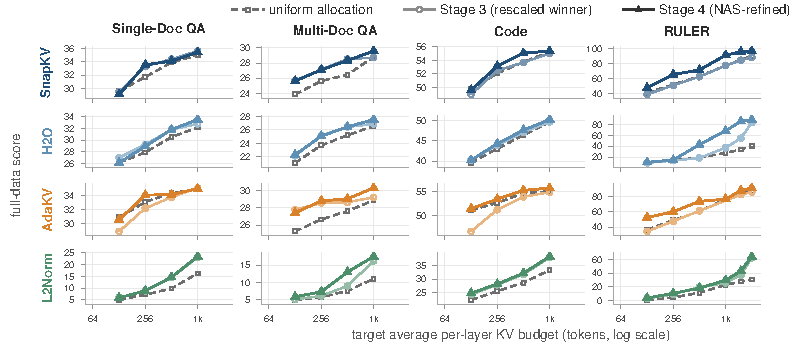
\includegraphics[width=0.845\textwidth]{figures/figure_stages_mistral.pdf}
  \caption{\textbf{Uniform vs.\ Stage 3 and Stage 4 at every target budget, Mistral-7B-Instruct-v0.2} (full data), drawn as Figure~\ref{fig:stages}. Rows: eviction method; columns: task. Stage 3: rescaled Stage 2 winner, no further search; Stage 4: NAS-refined, only at budgets where it ran.}
  \label{fig:app-stages-mistral}
\end{figure*}


\section{Calibration Scores vs.\ Full-Data Scores}
\label{app:calib}

MOSAIC scores configurations on a calibration subsample while it searches and on the full data when it selects. Figure~\ref{fig:app-calib} shows why both are needed: calibration orders configurations broadly like the full data, but the configuration it ranks first is often not the full-data best, and selection keeps only the first. The Stage 4 searches analysed here use a 10\% subsample for all four methods on both benchmarks; Stage 1 uses 30\% on LongBench and 10\% on RULER.

\paragraph{Stage 4 (Figure~\ref{fig:app-calib}a, b).} All candidates of a Stage 4 cell share one average budget, so their ranking tests calibration directly. Panel (a) gives Kendall's $\tau$ between the calibration and full-data rankings of each cell's re-evaluated candidates, and panel (b) the regret, the full-data points lost by taking the calibration-best candidate instead of the best re-evaluated one. On LongBench the median $\tau$ per method is 0.00 to 0.55, and calibration picks the full-data best in only 4 of 13 cells for SnapKV, 2 of 16 for H2O, 2 of 9 for AdaKV and 10 of 16 for L2Norm; on RULER it picks the full-data best in 20 of 21 cells (Table~\ref{tab:app-calib-summary}).

\paragraph{Stage 1 fronts (Figure~\ref{fig:app-calib}c, d).} Panels (c) and (d) compare each Stage 1 Pareto front's calibration scores with its Stage 2 full-data re-evaluation. On a front both scores rise with budget, so the front's overall order agrees ($\tau$ 0.78 to 1.00; in 15 of 17 fronts $\tau$ equals that between average budget and full-data score). Stage 2, however, keeps only the top configuration. The calibration-top configuration is the most expensive on the front in 15 of 17 fronts, and full data prefers a cheaper one in 6 of 17 (by up to 0.73 points; none of L2Norm's 4 LongBench fronts). For AdaKV, the Single- and Multi-Doc QA fronts are shown. Re-scoring a front costs only its 4 to 19 configurations.



\begin{table}[!htbp]
  \centering
  \footnotesize\setlength{\tabcolsep}{2.5pt}
  % Stage 4 calibration summary (10% subset); was main-text Table 1 until 2026-10-05, now in Appendix B
\begin{tabular}{@{} l l r r r r r @{}}
    \toprule
    \textbf{Bench.} & \textbf{Method} & \textbf{Cells} & \textbf{Gap} & \textbf{$\tau$} & \textbf{Picks} & \textbf{Regret} \\
    \midrule
    \rowcolor{gray!10}
    LongBench & H2O    & 16 & $+3.77$ & $-0.00$ & 2/16 & 0.71 \\
    LongBench & SnapKV & 13 & $+5.23$ & $+0.03$ & 4/13 & 0.60 \\
    \rowcolor{gray!10}
    RULER     & H2O    & 4  & $+0.09$ & $+0.82$ & 4/4  & 0.00 \\
    RULER     & SnapKV & 5  & $-0.16$ & $+1.00$ & 5/5  & 0.00 \\
    \midrule
    \rowcolor{gray!10}
    LongBench & AdaKV & 9 & $+1.14$ & $+0.47$ & 2/9 & 0.40 \\
    RULER     & AdaKV  & 6  & $-0.20$ & $+0.77$ & 5/6  & 0.02 \\
    \midrule
    \rowcolor{gray!10}
    LongBench & L2Norm & 16 & $+2.58$ & $+0.49$ & 10/16 & 0.30 \\
    RULER     & L2Norm & 6  & $+0.13$ & $+0.93$ & 6/6   & 0.00 \\
    \bottomrule
  \end{tabular}

  \caption{\textbf{Stage 4 calibration (10\% subset) vs.\ full-data scores, summary.} Cells: (task, budget) pairs. Gap: mean calibration minus full-data score. $\tau$: mean Kendall correlation between the two rankings of each cell's re-evaluated configurations. Picks: cells where the calibration-best candidate is also full-data best. Regret: mean full-data points lost by trusting calibration.}
  \label{tab:app-calib-summary}
\end{table}

\begin{figure*}[tp]
  \centering
  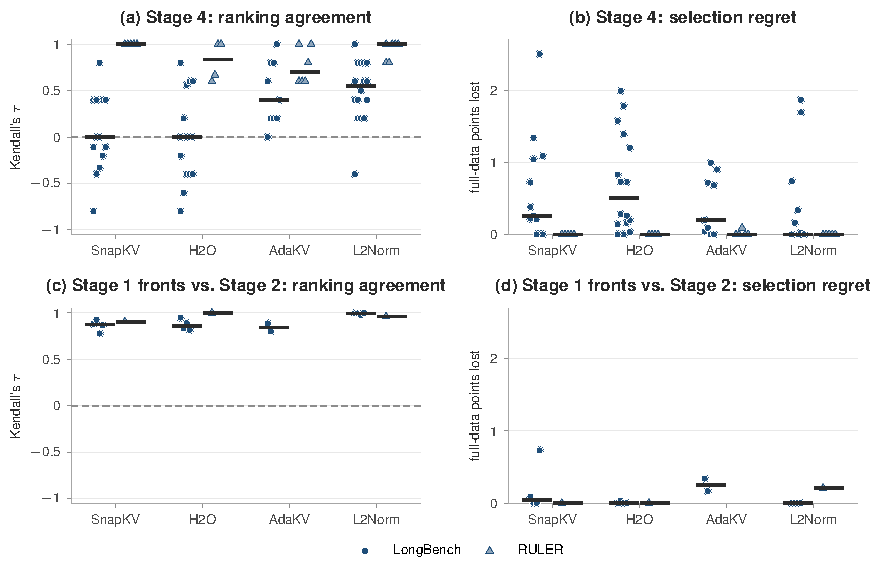
\includegraphics[width=0.92\textwidth]{figures/figure_calib.pdf}
  \caption{\textbf{Calibration vs.\ full-data scores, Llama-3-8B-Instruct.} Circles: LongBench; triangles: RULER; bars: medians. Top: Stage 4 (10\% subset on both benchmarks), one marker per evaluated (task, budget) cell, whose candidates share one budget. Bottom: Stage 1 Pareto fronts (30\% on LongBench, 10\% on RULER) against their Stage 2 full-data re-evaluation, one marker per front (AdaKV: Single- and Multi-Doc QA). (a, c) Kendall's $\tau$ between the calibration and full-data rankings. On a front both scores rise with budget, so (c) is high and in 15 of 17 fronts equals $\tau$ between average budget and full-data score: it reflects the budget trend, not whether calibration finds the top configuration. (b, d) Regret: full-data points lost by taking the calibration-top configuration instead of the best re-evaluated one. In (d), full data prefers a cheaper configuration than the calibration-top one in 6 of 17 fronts (up to 0.73 points). ``Best'' refers to the re-evaluated pool only, and a zero median regret does not mean calibration always picks correctly (Table~\ref{tab:app-calib-summary} gives the Stage 4 counts).}
  \label{fig:app-calib}
\end{figure*}


\paragraph{Calibration ratio: a case study.} Table~\ref{tab:app-calib-ratio} rescores the 24 configurations of one SnapKV Stage 4 search (Code, B512) on a 30\% subsample and compares both subsamples with the full data. In this cell the larger subsample reduces the optimism (+1.37 against +5.10 points), ranks the configurations closer to the full data ($\tau$ 0.75 against 0.51), and picks the full-data best, which the 10\% subsample does not. This is a single cell, chosen because its guided proposal scored below uniform, so it illustrates rather than establishes the effect; a 30\% subsample also costs about three times as much per evaluation. A larger subsample reduces the noise but does not remove it: on the Stage 1 fronts, which use 30\% on LongBench, full data prefers a different configuration from the calibration-top one in 4 of 15 SnapKV, H2O and L2Norm fronts (by up to 0.73 points; Figure~\ref{fig:app-calib}d). MOSAIC therefore re-evaluates its candidates on full data at either ratio.

\begin{table}[!htbp]
  \centering
  \footnotesize
  \setlength{\tabcolsep}{4pt}
  \begin{tabular}{@{}l r r c r@{}}
    \toprule
    Subsample & Gap & $\tau$ & Picks best & Regret \\
    \midrule
    10\% & +5.10 & +0.51 & no & 2.87 \\
    30\% & +1.37 & +0.75 & yes & 0.00 \\
    \bottomrule
  \end{tabular}
  \caption{\textbf{Calibration ratio, one cell} (SnapKV, Code B512, 24 configurations, full data as reference). Gap: mean calibration minus full-data score.}
  \label{tab:app-calib-ratio}
\end{table}


\section{Shape Transfer Across Tasks and Methods}
\label{app:transfer}


Figure~\ref{fig:app-shape-transfer} applies a Stage 2 winner shape to a different task or eviction method, rescaled with the same mapping as Stage 3, and compares it with the receiving cell's uniform allocation, its own rescaled Winner and its final configuration. The tests cover SnapKV and H2O on Code and Single-Doc QA at B128, B512 and B1024.

\textbf{Across tasks, shapes do not transfer.} SnapKV's Code shape applied to Single-Doc QA, and its Single-Doc QA shape applied to Code, score below uniform at every budget (by 0.33 to 1.08 and 0.63 to 1.22 points), while each task's own Winner beats uniform in the same six cells. The layers that need more cache differ between the two tasks, so a shape found for one task is worse than uniform allocation on the other.

\textbf{Across eviction methods, shapes do transfer.} On Code, H2O's shape under SnapKV and SnapKV's shape under H2O beat uniform in all six cells ($+0.06$ to $+1.66$). They stay below the receiving method's own final configuration in every cell (by 0.18 to 1.23 points) and below its own Winner in 4 of 6; SnapKV's shape under H2O beats H2O's own Winner at B128 and B1024 ($+0.16$ and $+0.90$). Which layers need more cache therefore depends mainly on the task, so a shape found with one eviction method is a useful starting point for another, while a search with the receiving method still adds up to 1.23 points.

\begin{figure*}[tp]
  \centering
  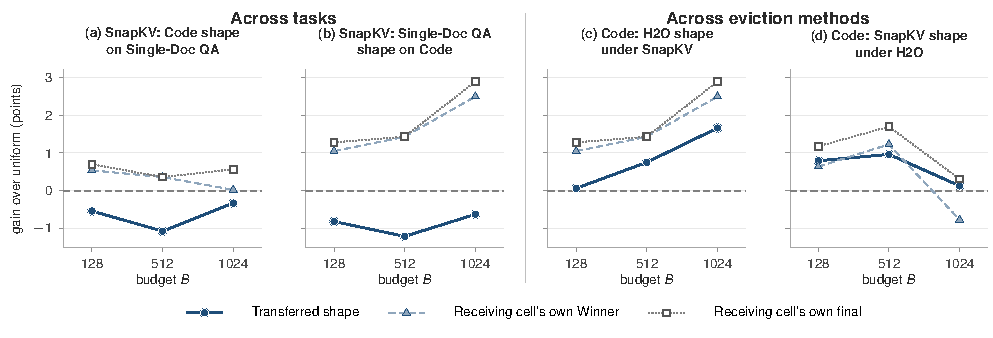
\includegraphics[width=0.95\textwidth]{figures/figure_transfer.pdf}
  \caption{\textbf{Transferring winner shapes across tasks (a, b) and eviction methods (c, d)}, LongBench, full data. Each point is a gain over the receiving cell's uniform allocation at the same budget (dashed line): the transferred shape, rescaled as in Stage 3; the receiving cell's own rescaled Winner; and its own final configuration (the better of Winner and NAS-refined).}
  \label{fig:app-shape-transfer}
\end{figure*}


\section{Search Cost}
\label{app:cost}

Table~\ref{tab:app-cost} compares one budget-constrained search per cell with our EvolKV reproduction (SnapKV, LongBench), on the same A100-40GB machine and evaluation harness. EvolKV runs 60 generations $\times$ population 10, 600 evaluations on 30 calibration samples each. MOSAIC's Stage 4 runs at most 150 evaluations on a 10\% calibration subset (55--100 samples): we keep each run's evaluations $\leq$150 in the order they were run, and add the full-data re-evaluation of the three NAS-refined candidates. Both searches process a sample equally fast (about 2.5\,s on Code and 1.0\,s on Single-Doc QA), so cost is evaluations times samples, and MOSAIC spends it on fewer evaluations of larger samples. It costs no more than EvolKV in any cell (43.8 GPU-hours against 53.7 in total) and beats it in 5 of 6 cells ($+0.17$ to $+1.71$); it loses Single-Doc QA B512 by 0.67 points.

MOSAIC has four stages. Stages 1--2 run once per (task, method) and produce the Winner; Stages 3--4 rescale it to each budget and refine it there. Users can stop after Stages 1--2 and deploy the rescaled Winner, which beats direct EvolKV in all 6 cells (Section~\ref{sec:evolkv}), or also run Stage 4 at the budgets they need. Stage 2 re-evaluates the Stage 1 front on full data: 3.6 GPU-hours on Single-Doc QA (20 configurations) and 8.0 on Code (11 configurations). Table~\ref{tab:app-step1} gives the cost of the 180-evaluation Stage 1 for each task and method. With Stages 1--2 added, running all four stages costs more than EvolKV's direct searches at these three budgets (at least 43.1 vs.\ 38.3 GPU-hours on Code, 21.2 vs.\ 15.4 on Single-Doc QA).



\begin{table}[H]
  \centering
  \small
  \setlength{\tabcolsep}{12pt}\renewcommand{\arraystretch}{1.2}
  \begin{tabular}{@{}l l r@{}}
    \toprule
    Category & Method & GPU-h \\
    \midrule
    SingleDoc & SnapKV & 9.0 \\
    SingleDoc & H2O & 26.0 \\
    MultiDoc & H2O & 29.4 \\
    RULER & SnapKV & 22.9 \\
    RULER & H2O & 39.7 \\
    \bottomrule
  \end{tabular}
  \caption{\textbf{MOSAIC Stage 1 cost}}
  \label{tab:app-step1}
\end{table}


\section{Choice of the Per-Layer Floor}
\label{app:floor}

SnapKV and H2O always retain an 8-token recent window, so a layer with budget $b$ selects only $b-8$ tokens by attention. At a floor of 16, only 8 tokens are chosen from contexts of thousands. Table~\ref{tab:app-floor} shows how often MOSAIC's final configuration in each cell places layers exactly at the floor. At B128, 8 to 24 of the 32 layers sit at the floor, so the floor matters most at low budgets, which is where the controlled comparison below finds its differences.

\begin{table}[H]
  \centering
  \footnotesize
  \setlength{\tabcolsep}{4pt}
  \begin{tabular}{@{}l l rrrr@{}}
    \toprule
    Task & Method & 128 & 256 & 512 & 1024 \\
    \midrule
    Code & SnapKV & 16 & 15 & 0 & 1 \\
     & H2O & 18 & 8 & 2 & 1 \\
    MultiDoc & SnapKV & 24 & 0 & 0 & 0 \\
     & H2O & 17 & 4 & 0 & 17 \\
    SingleDoc & SnapKV & 8 & 3 & 0 & 1 \\
     & H2O & 9 & 3 & 1 & 0 \\
    Summ & SnapKV & 8 & 6 & 0 & 0 \\
     & H2O & 13 & 6 & 0 & 0 \\
    RULER & SnapKV & 14 & 11 & 0 & 10 \\
     & H2O & 19 & 0 & 0 & 21 \\
    \bottomrule
  \end{tabular}
  \caption{\textbf{Layers at the per-layer floor (out of 32) in MOSAIC's final configuration of each cell.}}
  \label{tab:app-floor}
\end{table}


\paragraph{Controlled comparison.} Table~\ref{tab:app-floor-ablation} decodes the same rescaled SnapKV winner under both floors and evaluates both on full data. Floor 64 is better in three cells, all at B128 (by 0.37--1.10 points), the two are tied in two cells, and floor 16 is better in one (by 0.26). The differences concentrate at the lowest budget, where the floor binds most often.

\begin{table}[H]
  \centering
  \footnotesize
  \setlength{\tabcolsep}{3pt}
  \begin{tabular}{@{}l r r r r@{}}
    \toprule
    Cell & Uniform & Floor 64 & Floor 16 & $\Delta$ (16$-$64) \\
    \midrule
    Code B128 & 54.81 & 55.86 & 54.76 & \textbf{$-$1.10} \\
    Code B256 & 55.67 & 57.33 & 57.30 & \textbf{$-$0.02} \\
    SingleDoc B128 & 32.97 & 33.51 & 33.14 & \textbf{$-$0.37} \\
    SingleDoc B256 & 35.25 & 34.51 & 34.77 & +0.26 \\
    MultiDoc B128 & 34.82 & 35.02 & 34.32 & \textbf{$-$0.70} \\
    MultiDoc B256 & 35.60 & 36.31 & 36.31 & +0.00 \\
    \bottomrule
  \end{tabular}
  \caption{\textbf{Same rescaled winner under floor 64 and floor 16} (SnapKV, LongBench, full data). Negative $\Delta$ (bold): floor 64 is better.}
  \label{tab:app-floor-ablation}
\end{table}

\begin{table*}[tp]
  \centering
  \footnotesize
  \setlength{\tabcolsep}{4pt}
  \begin{tabular}{@{}l r r r r r r r r r r@{}}
    \toprule
    & & \multicolumn{4}{c}{EvolKV, direct} & \multicolumn{4}{c}{MOSAIC Stage 4, NAS-refined} & \\ \cmidrule(lr){3-6}\cmidrule(lr){7-10}
    Category & Budget & Evals & Samples & GPU-h & Score & Evals & Samples & GPU-h & Score & $\Delta$ \\
    \midrule
    Code & 128 & 601 & 30 & 12.7 & 54.92 & 150 & 100 & 12.6 & 55.73 & +0.81 \\
    Code & 512 & 601 & 30 & 12.9 & 57.02 & 148 & 100 & 12.0 & 58.01 & +0.99 \\
    Code & 1024 & 601 & 30 & 12.7 & 57.20 & 125 & 100 & 10.6 & 58.91 & +1.71 \\
    SingleDoc & 128 & 601 & 30 & 5.2 & 33.50 & 150 & 55 & 2.8 & 33.67 & +0.17 \\
    SingleDoc & 512 & 601 & 30 & 5.1 & 36.28 & 150 & 55 & 3.0 & 35.61 & \textbf{$-$0.67} \\
    SingleDoc & 1024 & 601 & 30 & 5.1 & 36.40 & 150 & 55 & 2.8 & 37.01 & +0.61 \\
    \textbf{Total} &  &  &  & \textbf{53.7} &  &  &  & \textbf{43.8} &  & \textbf{5/6} \\
    \bottomrule
  \end{tabular}
  \caption{\textbf{Per-budget search cost and score, EvolKV direct vs.\ MOSAIC Stage 4} (SnapKV, LongBench, full-data scores, A100). EvolKV: 600 evaluations plus one final evaluation. MOSAIC: $\leq$150 evaluations of each Stage 4 run; its GPU-hours include the full-data re-evaluation of three candidates but exclude the one-time Stages 1--2. $\Delta$: NAS-refined minus EvolKV; losses in bold.}
  \label{tab:app-cost}
\end{table*}


\section{AdaKV and L2Norm Per-Layer Allocations}
\label{app:adakv-shapes}

Figure~\ref{fig:app-adakv-shapes} is the AdaKV counterpart of Figure~\ref{fig:heatmap}, drawn in the same way. AdaKV shows a weaker version of the middle-layer preference: layer 10 receives more than its uniform share in 95\% of the 19 AdaKV allocations and layers 13--16 in 68--89\%, but over the whole middle block (layers 10 and 14--20) the share is 55\%, against 65\% for SnapKV and H2O. Figure~\ref{fig:app-l2norm-shapes} does the same for L2Norm. Its allocations favour layers 14--18, which receive more than their uniform share in 56--70\% of the 27 L2Norm allocations, and layer 27 (70\%); over the whole middle block the share is 51\%.

\begin{figure*}[tp]
  \centering
  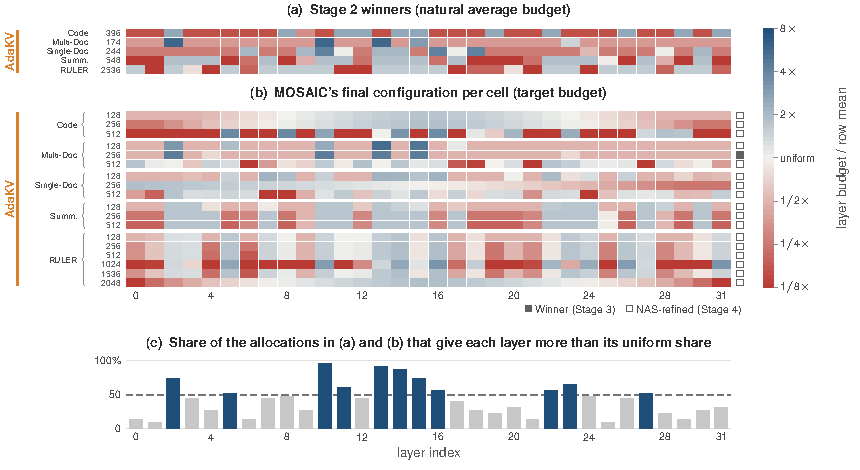
\includegraphics{figures/figure_adakv_layers.pdf}
  \caption{\textbf{AdaKV per-layer allocations}, drawn as Figure~\ref{fig:heatmap}. \textit{(a)} Stage 2 winners at their natural average budget (left). \textit{(b)} MOSAIC's final configuration for every cell (the better of Winner and NAS-refined), with the target budget on the left and a marker on the right for which of the two it is. \textit{(c)} For each layer, the share of the 19 allocations in (a) and (b) that give it more than its uniform share; navy bars exceed 50\%. Colour: each layer's budget divided by the row mean, on a log$_2$ scale (blue: more than the uniform share; red: less).}
  \label{fig:app-adakv-shapes}
\end{figure*}

\begin{figure*}[tp]
  \centering
  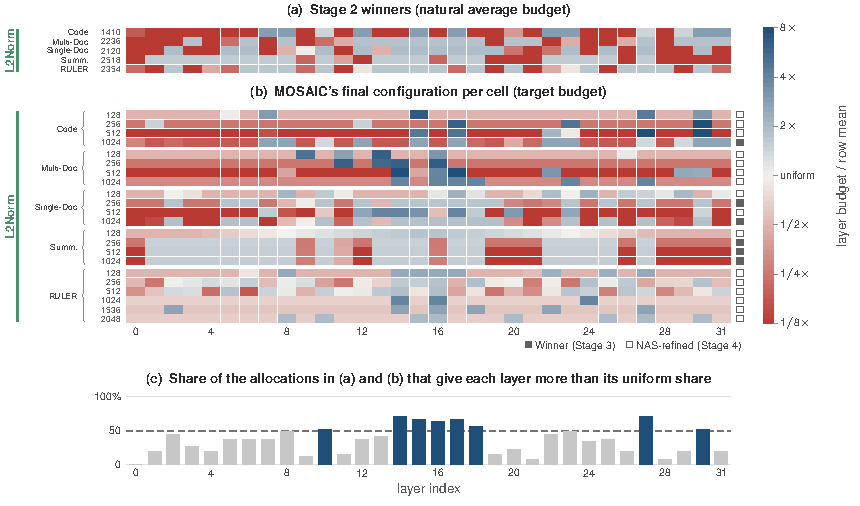
\includegraphics{figures/figure_l2norm_layers.pdf}
  \caption{\textbf{L2Norm per-layer allocations}, drawn as Figure~\ref{fig:heatmap}. \textit{(a)} Stage 2 winners at their natural average budget (left). \textit{(b)} MOSAIC's final configuration for every cell (the better of Winner and NAS-refined), with the target budget on the left and a marker on the right for which of the two it is. \textit{(c)} For each layer, the share of the 27 allocations in (a) and (b) that give it more than its uniform share; navy bars exceed 50\%. Colour: each layer's budget divided by the row mean, on a log$_2$ scale (blue: more than the uniform share; red: less).}
  \label{fig:app-l2norm-shapes}
\end{figure*}

\begin{figure*}[tp]
  \centering
  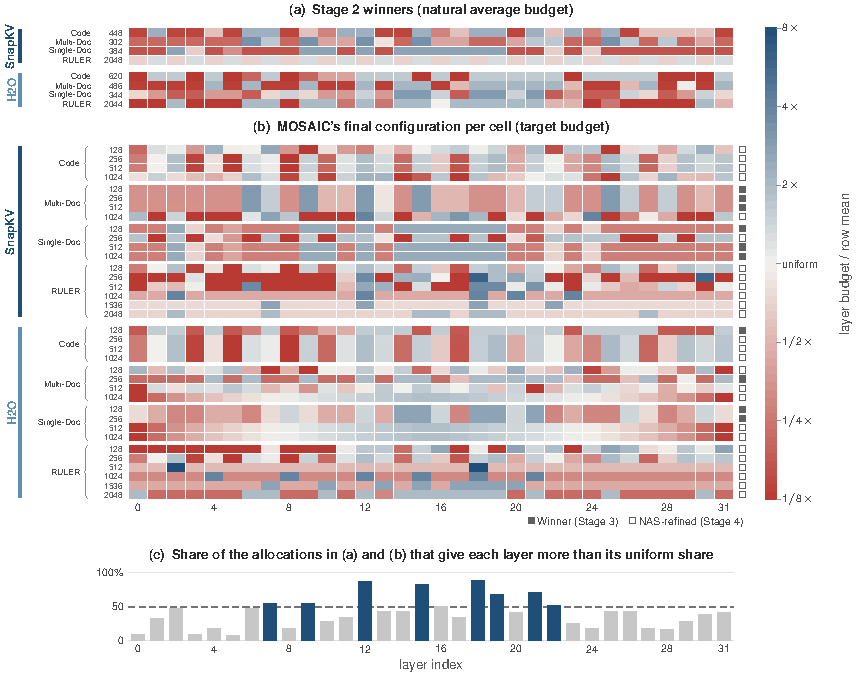
\includegraphics{figures/figure_mistral_snapkv_h2o_layers.pdf}
  \caption{\textbf{SnapKV and H2O per-layer allocations, Mistral-7B-Instruct-v0.2}, drawn as Figure~\ref{fig:heatmap}. \textit{(a)} Stage 2 winners at their natural average budget (left). \textit{(b)} MOSAIC's final configuration for every cell (the better of Winner and NAS-refined), with the target budget on the left and a marker on the right for which of the two it is. \textit{(c)} For each layer, the share of the 44 allocations in (a) and (b) that give it more than its uniform share; navy bars exceed 50\%. Colour: each layer's budget divided by the row mean, on a log$_2$ scale (blue: more than the uniform share; red: less).}
  \label{fig:app-mistral-shapes}
\end{figure*}

\begin{figure*}[tp]
  \centering
  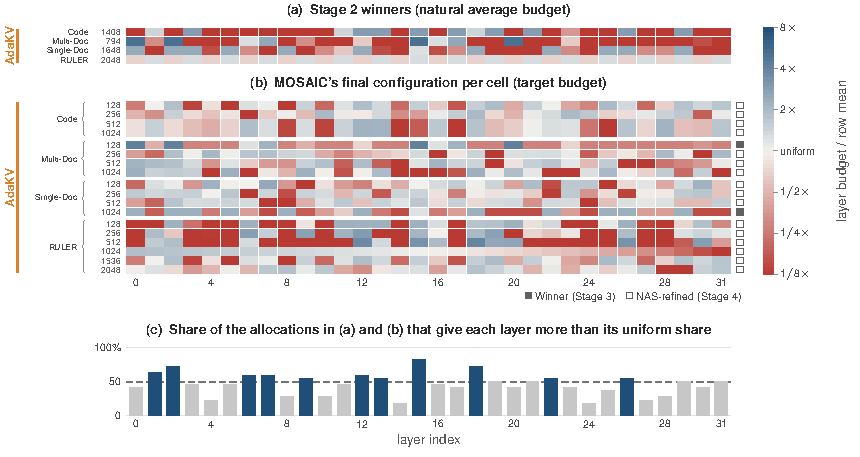
\includegraphics{figures/figure_mistral_adakv_layers.pdf}
  \caption{\textbf{AdaKV per-layer allocations, Mistral-7B-Instruct-v0.2}, drawn as Figure~\ref{fig:heatmap}. \textit{(a)} Stage 2 winners at their natural average budget (left). \textit{(b)} MOSAIC's final configuration for every cell (the better of Winner and NAS-refined), with the target budget on the left and a marker on the right for which of the two it is. \textit{(c)} For each layer, the share of the 22 allocations in (a) and (b) that give it more than its uniform share; navy bars exceed 50\%. Colour: each layer's budget divided by the row mean, on a log$_2$ scale (blue: more than the uniform share; red: less).}
  \label{fig:app-mistral-adakv-shapes}
\end{figure*}

\begin{figure*}[tp]
  \centering
  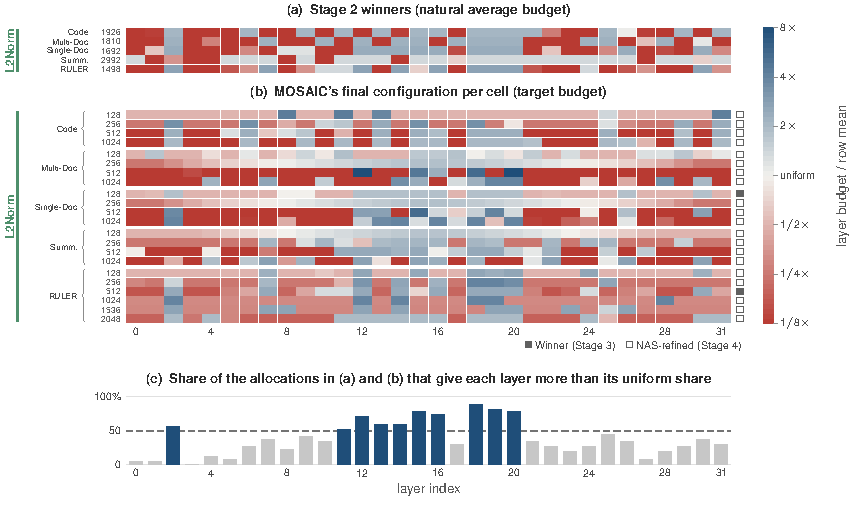
\includegraphics{figures/figure_mistral_l2norm_layers.pdf}
  \caption{\textbf{L2Norm per-layer allocations, Mistral-7B-Instruct-v0.2}, drawn as Figure~\ref{fig:heatmap}. \textit{(a)} Stage 2 winners at their natural average budget (left). \textit{(b)} MOSAIC's final configuration for every cell (the better of Winner and NAS-refined), with the target budget on the left and a marker on the right for which of the two it is. \textit{(c)} For each layer, the share of the 27 allocations in (a) and (b) that give it more than its uniform share; navy bars exceed 50\%. Colour: each layer's budget divided by the row mean, on a log$_2$ scale (blue: more than the uniform share; red: less).}
  \label{fig:app-mistral-l2norm-shapes}
\end{figure*}


\section{Further Related Work}
\label{app:related}

\textbf{Complementary cache compression.} Other techniques shrink the KV cache along axes that per-layer allocation leaves untouched and can be combined with it: Quest \citep{tang2024quest} keeps the full cache but loads only the pages relevant to each query, KIVI \citep{liu2024kivi} and KVQuant \citep{hooper2024kvquant} quantize keys and values to a few bits, and MiniCache \citep{liu2024minicache} merges the caches of adjacent layers.

\textbf{Searching once for many budgets.} Once-for-All \citep{cai2020ofa} trains one network and specializes it to many hardware budgets; MOSAIC similarly searches once and rescales the result to many cache budgets. Gradient-based NAS such as DARTS \citep{liu2019darts} does not apply here, because the task score is not differentiable in the per-layer token budgets.

\section{Reproducibility Details}
\label{app:repro}

Algorithm~\ref{alg:mosaic} summarizes the MOSAIC pipeline for one (task, eviction method); the paragraphs below give its settings.

\begin{algorithm}[t]
\caption{MOSAIC for one (task, eviction method).}
\label{alg:mosaic}
\footnotesize
\begin{algorithmic}[1]
\Require calibration subset $D_{\mathrm{cal}}$, full data $D_{\mathrm{full}}$, target budgets $\mathcal{B}$, Stage 1 grid $G$, evaluation cap $N$
\State \textit{Stage 1:} $A \gets$ uniform allocation at every level of $G$ $\cup$ Latin Hypercube points \Comment{64 points}
\State $A \gets \textsc{GuidedSearch}(A$, minimize average budget, maximize score on $D_{\mathrm{cal}})$
\State $P \gets$ Pareto front of $A$
\State \textit{Stage 2:} $w \gets$ the non-uniform $p \in P$ with the highest score on $D_{\mathrm{full}}$
\For{each target budget $B \in \mathcal{B}$}
  \State \textit{Stage 3:} $b_W \gets \textsc{Rescale}(w, B)$ \Comment{Winner}
  \State \textit{Stage 4 (optional):} $A_B \gets \{$uniform, 5 heuristic shapes, $b_W$, 57 LHS points$\}$, all with mean budget $B$
  \State $A_B \gets \textsc{GuidedSearch}(A_B$, maximize score on $D_{\mathrm{cal}})$
  \State $C \gets$ the calibration-best candidates of $A_B \setminus \{$uniform, $b_W\}$
  \State $b_N \gets$ the $c \in C$ with the highest score on $D_{\mathrm{full}}$ \Comment{NAS-refined}
  \State final configuration at $B \gets$ the better of $b_W$ and $b_N$ on $D_{\mathrm{full}}$
\EndFor
\Statex
\Procedure{GuidedSearch}{$A$, objectives}
  \Repeat
    \State rank $A$ by non-dominated sorting on the objectives
    \State train an MLP classifier to separate rank-1 configurations from the rest
    \State $\mathbf{x}^* \gets \arg\max_{\mathbf{x}} P(\mathrm{rank}\ 1 \mid \mathbf{x})$, by differential evolution
    \State evaluate $\mathbf{x}^*$ on $D_{\mathrm{cal}}$; \ $A \gets A \cup \{\mathbf{x}^*\}$
  \Until{the search stops improving or $|A| = N$}
  \State \Return $A$
\EndProcedure
\end{algorithmic}
\end{algorithm}

\paragraph{Budget decoding.} Stage 1 maps each coordinate $x_i \in [0,1]$ of a configuration to a discrete per-layer budget by equal-width bins over a grid $G$: seven levels from 64 to 4096 on RULER and in some LongBench runs, and five levels from 64 to 1024 in the other LongBench runs. The grid limits only Stage 1: Stages 3 and 4 decode continuously between the floor and 4096, scaling the weights $x_i$ to the total $T = 32B$, clamping layers at the cap and the floor and redistributing the remainder in proportion to $x_i$, then rounding so that $\sum_i b_i = T$ exactly. \emph{Search-space size.} The Stage 1 grid holds $|G|^{32}$ configurations ($5^{32} \approx 2.3\times10^{22}$ or $7^{32} \approx 1.1\times10^{27}$) across all average budgets. Stage 4 searches integer allocations in $[64, 4096]^{32}$ at a fixed budget $B$: about $7\times10^{68}$ at B128, and $10^{84}$, $10^{95}$, $10^{105}$ and $10^{111}$ at B256, B512, B1024 and B2048. One EvolKV search varies a single 8-layer group with the others fixed, so even ignoring its budget penalty it covers at most $4033^8 \approx 7\times10^{28}$ allocations, about $10^{40}$ times fewer than one MOSAIC search at B128. This compares single searches: the allocations of both methods lie in the same space $[64, 4096]^{32}$.

\paragraph{Rescaling the Stage 2 winner.} A winner with per-layer budgets $w_i$ is mapped to $x_i = 0.05 + 0.9\,w_i / \max_j w_j$ and decoded at each target $B$ as above; this keeps the order of the layers and the shape of the allocation but compresses the ratios between layers. The same mapping seeds the winner into the Stage 4 search.

\paragraph{Per-layer floor and cap.} The per-layer cap is 4096. Stage 1's grid maximum is 1024 for most LongBench runs and 4096 for RULER; Stages 3 and 4 decode continuously between the floor (64 or 16) and the cap (4096). Table~\ref{tab:app-floor} reports how often the floor binds.

\paragraph{Stopping rules.} Searches were capped at 180  evaluations in Stage 1, 150 evaluations in Stage 4 and were stopped earlier, by hand or when the best calibration score stopped improving, so run lengths vary across methods and cells.

\paragraph{Candidate provenance.} Stage 2 re-evaluates configurations from the Stage 1 Pareto front on full data and takes the best non-uniform one as the Winner. Stage 4 re-evaluates on full data uniform, the Winner and the calibration-best of the search's other candidates (heuristic shapes, LHS points and guided proposals). NAS-refined is the best of these other candidates, so it excludes uniform and the Winner and can score below the Winner; MOSAIC's final configuration is the better of the two.

\paragraph{Stage 4 initial design.} Each Stage 4 search starts from 64 configurations at the target budget: uniform, five heuristic shapes (ascending and descending ramps, a middle-heavy triangle, its inverse, and alternating low/high layers), the Winner, and 57 Latin hypercube points, which serve as a random-allocation control. Every later evaluation is one configuration proposed by \textsc{GuidedSearch}.

\paragraph{EvolKV baseline (expanded).} To reproduce EvolKV's main protocol, the allocation $k_i$ that our EvolKV run finds at B128 is expanded to each target $B$ with EvolKV's budget completion rule \citep{yu2025evolkv}, $b_i = k_i\,T / \sum_j k_j$, rounded so that the mean is exactly $B$ and clipped to $[64, 4096]$ (neither bound binds for B256--B1024).

\paragraph{Hardware.} Experiments ran on NVIDIA A100 GPUs, with FlashAttention-2 \citep{dao2024flashattention2} as the attention implementation for every method.


\section{Subtask and Dataset Breakdown}
\label{app:breakdown}

This section breaks the per-cell results of Appendix~\ref{app:cells} into RULER subtasks and LongBench datasets, comparing uniform allocation with MOSAIC's final configuration (the better of Winner and NAS-refined) in every cell; bold marks the better of the two in each column.


\subsection{RULER Subtask Breakdown}
\label{app:ruler}

Tables~\ref{tab:app-ruler} (Llama-3-8B-Instruct) and~\ref{tab:app-ruler-mistral} (Mistral-7B-Instruct-v0.2) break each RULER cell into its 11 subtasks (S1--3: niah\_single; MK1--3: niah\_multikey; MQ: multiquery; MV: multivalue; CWE/FWE: common/frequent-word extraction; VT: variable tracking; NIAH: mean of the eight needle subtasks; All: mean of all 11), comparing uniform with MOSAIC's final configuration; Figures~\ref{fig:app-heat-ruler} and~\ref{fig:app-heat-ruler-mistral} show the same gains as heatmaps. Averaged over floor-clean cells (floor 64, plus B1536/B2048), NAS gains concentrate on the hardest needle subtasks: MK3 +31.9, S3 +28.0, S1 +23.8, versus CWE +0.8, FWE +3.5 and VT +5.6. The floor-16 H2O B1024 configuration trades CWE accuracy (98.3$\rightarrow$21.5) for needle retrieval.


For AdaKV the pattern matches SnapKV and H2O: the largest gains are on niah\_multikey\_3 at B1024 and above.

\begin{figure*}[tp]
  \centering
  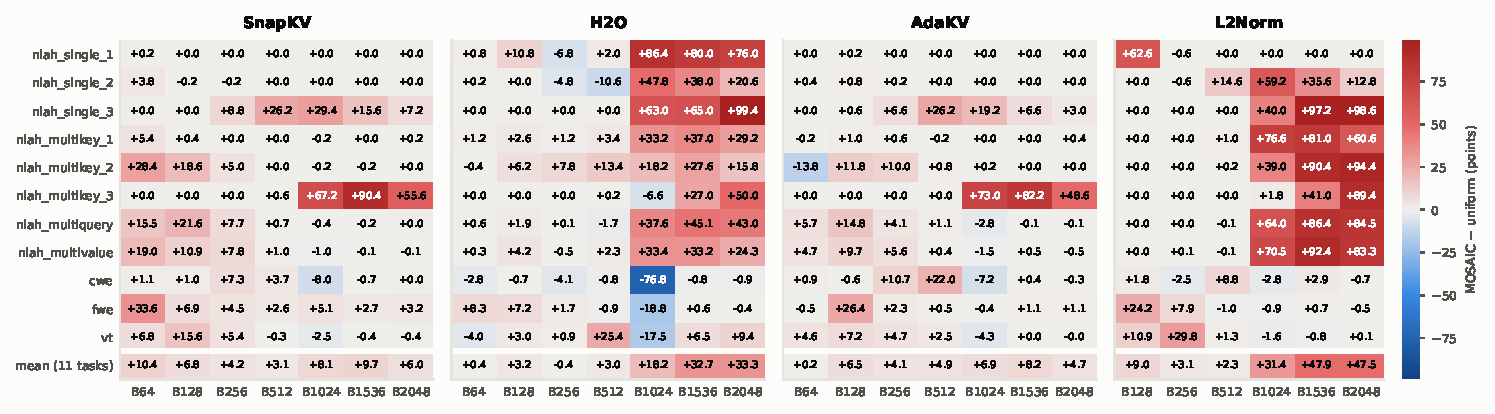
\includegraphics[width=\textwidth]{figures/figure_heat_ruler.pdf}
  \caption{\textbf{RULER subtask gains of MOSAIC over uniform, Llama-3-8B-Instruct} (the $\Delta$ rows of Table~\ref{tab:app-ruler}, points). Rows: subtasks and their mean; columns: budget. Red: MOSAIC above uniform; blue: below.}
  \label{fig:app-heat-ruler}
\end{figure*}

\begin{table*}[tp]
  \centering
  \scriptsize
  \setlength{\tabcolsep}{4pt}
  \renewcommand{\arraystretch}{0.92}
  \begin{tabular}{@{} c l rrrrrrrrrrrrr @{}}
    \toprule
    \textbf{Budget} & & \textbf{S1} & \textbf{S2} & \textbf{S3} & \textbf{MK1} & \textbf{MK2} & \textbf{MK3} & \textbf{MQ} & \textbf{MV} & \textbf{CWE} & \textbf{FWE} & \textbf{VT} & \textbf{NIAH} & \textbf{All} \\
    \midrule
    \multicolumn{15}{c}{\textbf{SnapKV}} \\
    \midrule
    \multirow{2}{*}{64} & Uniform & 99.8 & 93.4 & 0.0 & 91.2 & 48.0 & 0.0 & 7.9 & 17.0 & 1.8 & 1.3 & 20.6 & 44.7 & 34.6 \\
     & MOSAIC & \textbf{100.0} & \textbf{97.2} & 0.0 & \textbf{96.6} & \textbf{76.4} & 0.0 & \textbf{23.4} & \textbf{36.0} & \textbf{2.9} & \textbf{34.9} & \textbf{27.4} & \textbf{53.7} & \textbf{45.0} \\
    \cmidrule(l){1-15}
    \multirow{2}{*}{128} & Uniform & 100.0 & \textbf{98.6} & 0.2 & 98.0 & 72.8 & 0.0 & 36.2 & 53.1 & 8.2 & 49.5 & 50.6 & 57.4 & 51.6 \\
     & MOSAIC & 100.0 & 98.4 & 0.2 & \textbf{98.4} & \textbf{91.4} & 0.0 & \textbf{57.8} & \textbf{64.0} & \textbf{9.3} & \textbf{56.4} & \textbf{66.1} & \textbf{63.8} & \textbf{58.4} \\
    \cmidrule(l){1-15}
    \multirow{2}{*}{256} & Uniform & 100.0 & \textbf{99.8} & 1.4 & 99.4 & 93.0 & 0.0 & 82.5 & 84.5 & 30.8 & 68.0 & 89.3 & 70.1 & 68.1 \\
     & MOSAIC & 100.0 & 99.6 & \textbf{10.2} & 99.4 & \textbf{98.0} & 0.0 & \textbf{90.2} & \textbf{92.3} & \textbf{38.0} & \textbf{72.5} & \textbf{94.7} & \textbf{73.7} & \textbf{72.3} \\
    \cmidrule(l){1-15}
    \multirow{2}{*}{512} & Uniform & 100.0 & 100.0 & 23.4 & 99.4 & 99.6 & 0.0 & 97.8 & 96.5 & 73.4 & 78.7 & \textbf{96.2} & 77.1 & 78.6 \\
     & MOSAIC & 100.0 & 100.0 & \textbf{49.6} & 99.4 & 99.6 & \textbf{0.6} & \textbf{98.5} & \textbf{97.5} & \textbf{77.1} & \textbf{81.3} & 95.8 & \textbf{80.6} & \textbf{81.8} \\
    \cmidrule(l){1-15}
    \multirow{2}{*}{1024} & Uniform & 100.0 & 100.0 & 64.8 & \textbf{99.4} & \textbf{99.8} & 0.6 & \textbf{99.8} & \textbf{98.8} & \textbf{96.1} & 84.7 & \textbf{98.4} & 82.9 & 85.7 \\
     & MOSAIC & 100.0 & 100.0 & \textbf{94.2} & 99.2 & 99.6 & \textbf{67.8} & 99.3 & 97.8 & 88.2 & \textbf{89.8} & 95.9 & \textbf{94.7} & \textbf{93.8} \\
    \cmidrule(l){1-15}
    \multirow{2}{*}{1536} & Uniform & 100.0 & 100.0 & 83.8 & 99.4 & \textbf{100.0} & 6.8 & \textbf{100.0} & 98.8 & \textbf{99.0} & 88.1 & \textbf{98.9} & 86.1 & 88.6 \\
     & MOSAIC & 100.0 & 100.0 & \textbf{99.4} & 99.4 & 99.8 & \textbf{97.2} & 99.8 & 98.8 & 98.3 & \textbf{90.9} & 98.4 & \textbf{99.3} & \textbf{98.4} \\
    \cmidrule(l){1-15}
    \multirow{2}{*}{2048} & Uniform & 100.0 & 100.0 & 92.8 & 99.4 & 100.0 & 43.0 & 99.9 & \textbf{98.9} & 99.6 & 89.4 & \textbf{99.2} & 91.8 & 92.9 \\
     & MOSAIC & 100.0 & 100.0 & \textbf{100.0} & \textbf{99.6} & 100.0 & \textbf{98.6} & 99.9 & 98.8 & 99.6 & \textbf{92.6} & 98.9 & \textbf{99.6} & \textbf{98.9} \\
    \midrule
    \multicolumn{15}{c}{\textbf{H2O}} \\
    \midrule
    \multirow{2}{*}{64} & Uniform & 0.2 & 0.6 & 0.0 & 0.4 & \textbf{1.4} & 0.0 & 0.1 & 0.3 & \textbf{11.3} & 58.9 & \textbf{6.2} & 0.4 & 7.2 \\
     & MOSAIC & \textbf{1.0} & \textbf{0.8} & 0.0 & \textbf{1.6} & 1.0 & 0.0 & \textbf{0.8} & \textbf{0.6} & 8.5 & \textbf{67.2} & 2.2 & \textbf{0.7} & \textbf{7.6} \\
    \cmidrule(l){1-15}
    \multirow{2}{*}{128} & Uniform & 2.8 & 2.8 & 0.0 & 4.8 & 4.6 & 0.0 & 1.8 & 1.8 & \textbf{30.3} & 78.9 & 6.4 & 2.3 & 12.2 \\
     & MOSAIC & \textbf{13.6} & 2.8 & 0.0 & \textbf{7.4} & \textbf{10.8} & 0.0 & \textbf{3.7} & \textbf{5.9} & 29.6 & \textbf{86.1} & \textbf{9.4} & \textbf{5.5} & \textbf{15.4} \\
    \cmidrule(l){1-15}
    \multirow{2}{*}{256} & Uniform & \textbf{9.2} & \textbf{11.6} & 0.0 & 13.4 & 16.2 & 0.2 & 6.6 & \textbf{7.1} & \textbf{58.1} & 88.2 & 9.6 & \textbf{8.0} & \textbf{20.0} \\
     & MOSAIC & 2.4 & 6.8 & 0.0 & \textbf{14.6} & \textbf{24.0} & 0.2 & \textbf{6.7} & 6.6 & 54.0 & \textbf{89.9} & \textbf{10.5} & 7.7 & 19.6 \\
    \cmidrule(l){1-15}
    \multirow{2}{*}{512} & Uniform & 6.4 & \textbf{25.0} & 0.0 & 24.2 & 35.2 & 1.4 & \textbf{14.4} & 14.3 & \textbf{86.1} & \textbf{94.3} & 24.6 & 15.1 & 29.6 \\
     & MOSAIC & \textbf{8.4} & 14.4 & 0.0 & \textbf{27.6} & \textbf{48.6} & \textbf{1.6} & 12.8 & \textbf{16.6} & 85.3 & 93.4 & \textbf{50.1} & \textbf{16.2} & \textbf{32.6} \\
    \cmidrule(l){1-15}
    \multirow{2}{*}{1024} & Uniform & 10.2 & 44.2 & 0.0 & 47.0 & 57.6 & \textbf{7.6} & 24.8 & 30.4 & \textbf{98.3} & \textbf{96.3} & \textbf{71.6} & 27.7 & 44.4 \\
     & MOSAIC & \textbf{96.6} & \textbf{92.0} & \textbf{63.0} & \textbf{80.2} & \textbf{75.8} & 1.0 & \textbf{62.4} & \textbf{63.7} & 21.5 & 77.5 & 54.1 & \textbf{66.8} & \textbf{62.5} \\
    \cmidrule(l){1-15}
    \multirow{2}{*}{1536} & Uniform & 16.2 & 58.8 & 0.0 & 61.0 & 71.8 & 24.6 & 35.6 & 44.4 & \textbf{99.3} & 95.1 & 80.4 & 39.0 & 53.4 \\
     & MOSAIC & \textbf{96.2} & \textbf{96.8} & \textbf{65.0} & \textbf{98.0} & \textbf{99.4} & \textbf{51.6} & \textbf{80.8} & \textbf{77.6} & 98.5 & \textbf{95.7} & \textbf{86.9} & \textbf{83.2} & \textbf{86.0} \\
    \cmidrule(l){1-15}
    \multirow{2}{*}{2048} & Uniform & 24.0 & 79.4 & 0.0 & 70.4 & 83.2 & 48.6 & 47.6 & 58.0 & \textbf{99.6} & \textbf{95.1} & 85.0 & 51.4 & 62.8 \\
     & MOSAIC & \textbf{100.0} & \textbf{100.0} & \textbf{99.4} & \textbf{99.6} & \textbf{99.0} & \textbf{98.6} & \textbf{90.7} & \textbf{82.3} & 98.8 & 94.7 & \textbf{94.5} & \textbf{96.2} & \textbf{96.1} \\
    \midrule
    \multicolumn{15}{c}{\textbf{AdaKV}} \\
    \midrule
    \multirow{2}{*}{64} & Uniform & 99.6 & 92.0 & 0.0 & \textbf{91.6} & \textbf{51.6} & 0.0 & 8.2 & 26.7 & 4.0 & \textbf{0.7} & 19.4 & \textbf{46.2} & 35.8 \\
     & MOSAIC & 99.6 & \textbf{92.4} & 0.0 & 91.4 & 37.8 & 0.0 & \textbf{13.9} & \textbf{31.4} & \textbf{4.9} & 0.2 & \textbf{24.0} & 45.8 & \textbf{36.0} \\
    \cmidrule(l){1-15}
    \multirow{2}{*}{128} & Uniform & 99.8 & 97.8 & 0.0 & 97.4 & 68.2 & 0.0 & 44.2 & 65.8 & \textbf{15.3} & 16.8 & 54.2 & 59.1 & 50.9 \\
     & MOSAIC & \textbf{100.0} & \textbf{98.6} & \textbf{0.6} & \textbf{98.4} & \textbf{80.0} & 0.0 & \textbf{59.0} & \textbf{75.5} & 14.7 & \textbf{43.2} & \textbf{61.5} & \textbf{64.0} & \textbf{57.4} \\
    \cmidrule(l){1-15}
    \multirow{2}{*}{256} & Uniform & 100.0 & 99.8 & 4.2 & 98.8 & 84.8 & 0.0 & 89.5 & 90.4 & 28.9 & 68.1 & 83.7 & 70.9 & 68.0 \\
     & MOSAIC & 100.0 & \textbf{100.0} & \textbf{10.8} & \textbf{99.4} & \textbf{94.8} & 0.0 & \textbf{93.5} & \textbf{96.0} & \textbf{39.7} & \textbf{70.4} & \textbf{88.4} & \textbf{74.3} & \textbf{72.1} \\
    \cmidrule(l){1-15}
    \multirow{2}{*}{512} & Uniform & 100.0 & 100.0 & 32.6 & \textbf{99.6} & 97.4 & 0.0 & 98.5 & 97.3 & 59.0 & 81.9 & 94.2 & 78.2 & 78.2 \\
     & MOSAIC & 100.0 & 100.0 & \textbf{58.8} & 99.4 & \textbf{98.2} & 0.0 & \textbf{99.6} & \textbf{97.8} & \textbf{81.0} & \textbf{82.4} & \textbf{96.6} & \textbf{81.7} & \textbf{83.1} \\
    \cmidrule(l){1-15}
    \multirow{2}{*}{1024} & Uniform & 100.0 & 100.0 & 77.4 & 99.6 & 99.2 & 1.6 & \textbf{99.8} & \textbf{98.0} & \textbf{93.6} & \textbf{87.3} & \textbf{98.9} & 84.5 & 86.9 \\
     & MOSAIC & 100.0 & 100.0 & \textbf{96.6} & 99.6 & \textbf{99.4} & \textbf{74.6} & 97.0 & 96.5 & 86.4 & 86.9 & 94.6 & \textbf{95.5} & \textbf{93.8} \\
    \cmidrule(l){1-15}
    \multirow{2}{*}{1536} & Uniform & 100.0 & 100.0 & 91.2 & 99.6 & 100.0 & 10.6 & \textbf{99.9} & 98.3 & 98.7 & 89.7 & 99.1 & 87.5 & 89.7 \\
     & MOSAIC & 100.0 & 100.0 & \textbf{97.8} & 99.6 & 100.0 & \textbf{92.8} & 99.8 & \textbf{98.8} & \textbf{99.2} & \textbf{90.8} & 99.1 & \textbf{98.6} & \textbf{98.0} \\
    \cmidrule(l){1-15}
    \multirow{2}{*}{2048} & Uniform & 100.0 & 100.0 & 96.6 & 99.4 & 100.0 & 48.8 & \textbf{99.9} & \textbf{98.5} & \textbf{99.6} & 90.9 & \textbf{99.3} & 92.9 & 93.9 \\
     & MOSAIC & 100.0 & 100.0 & \textbf{99.6} & \textbf{99.8} & 100.0 & \textbf{97.4} & 99.8 & 98.0 & 99.3 & \textbf{91.9} & 99.2 & \textbf{99.3} & \textbf{98.6} \\
    \midrule
    \multicolumn{15}{c}{\textbf{L2Norm}} \\
    \midrule
    \multirow{2}{*}{128} & Uniform & 28.2 & 0.0 & 0.0 & 0.0 & 0.0 & 0.0 & 0.0 & 0.0 & 7.1 & 15.0 & 0.6 & 3.5 & 4.6 \\
     & MOSAIC & \textbf{90.8} & 0.0 & 0.0 & 0.0 & 0.0 & 0.0 & 0.0 & 0.0 & \textbf{9.0} & \textbf{39.2} & \textbf{11.6} & \textbf{11.3} & \textbf{13.7} \\
    \cmidrule(l){1-15}
    \multirow{2}{*}{256} & Uniform & \textbf{99.6} & \textbf{1.0} & 0.0 & 0.0 & 0.0 & 0.0 & 0.0 & 0.0 & \textbf{18.5} & 44.9 & 31.0 & \textbf{12.6} & 17.7 \\
     & MOSAIC & 99.0 & 0.4 & 0.0 & 0.0 & 0.0 & 0.0 & 0.0 & \textbf{0.1} & 16.0 & \textbf{52.9} & \textbf{60.8} & 12.4 & \textbf{20.8} \\
    \cmidrule(l){1-15}
    \multirow{2}{*}{512} & Uniform & 100.0 & 5.6 & 0.0 & 0.4 & 0.2 & 0.0 & \textbf{0.1} & \textbf{0.1} & 35.9 & \textbf{64.2} & 92.4 & 13.3 & 27.2 \\
     & MOSAIC & 100.0 & \textbf{20.2} & 0.0 & \textbf{1.4} & \textbf{0.4} & 0.0 & 0.0 & 0.0 & \textbf{44.8} & 63.2 & \textbf{93.6} & \textbf{15.2} & \textbf{29.4} \\
    \cmidrule(l){1-15}
    \multirow{2}{*}{1024} & Uniform & 100.0 & 32.0 & 0.2 & 5.4 & 1.4 & 0.4 & 0.2 & 0.2 & \textbf{73.6} & \textbf{79.1} & \textbf{99.0} & 17.5 & 35.6 \\
     & MOSAIC & 100.0 & \textbf{91.2} & \textbf{40.2} & \textbf{82.0} & \textbf{40.4} & \textbf{2.2} & \textbf{64.2} & \textbf{70.8} & 70.8 & 78.1 & 97.4 & \textbf{61.4} & \textbf{67.0} \\
    \cmidrule(l){1-15}
    \multirow{2}{*}{1536} & Uniform & 100.0 & 64.0 & 0.0 & 16.4 & 2.0 & 1.4 & 2.1 & 2.8 & 92.8 & 84.4 & \textbf{99.2} & 23.6 & 42.3 \\
     & MOSAIC & 100.0 & \textbf{99.6} & \textbf{97.2} & \textbf{97.4} & \textbf{92.4} & \textbf{42.4} & \textbf{88.6} & \textbf{95.2} & \textbf{95.7} & \textbf{85.1} & 98.4 & \textbf{89.1} & \textbf{90.2} \\
    \cmidrule(l){1-15}
    \multirow{2}{*}{2048} & Uniform & 100.0 & 87.0 & 1.4 & 38.4 & 3.8 & 5.8 & 12.1 & 13.2 & \textbf{97.9} & \textbf{87.8} & 99.2 & 32.7 & 49.7 \\
     & MOSAIC & 100.0 & \textbf{99.8} & \textbf{100.0} & \textbf{99.0} & \textbf{98.2} & \textbf{95.2} & \textbf{96.6} & \textbf{96.5} & 97.3 & 87.3 & \textbf{99.3} & \textbf{98.2} & \textbf{97.2} \\
    \bottomrule
  \end{tabular}
  \caption{\textbf{RULER subtask accuracy (string match, \%), uniform vs.\ MOSAIC per cell, Llama-3-8B-Instruct.} AdaKV B64 has only the rescaled winner, compared with uniform-64 from Stage 2.}
  \label{tab:app-ruler}
\end{table*}

\begin{figure*}[tp]
  \centering
  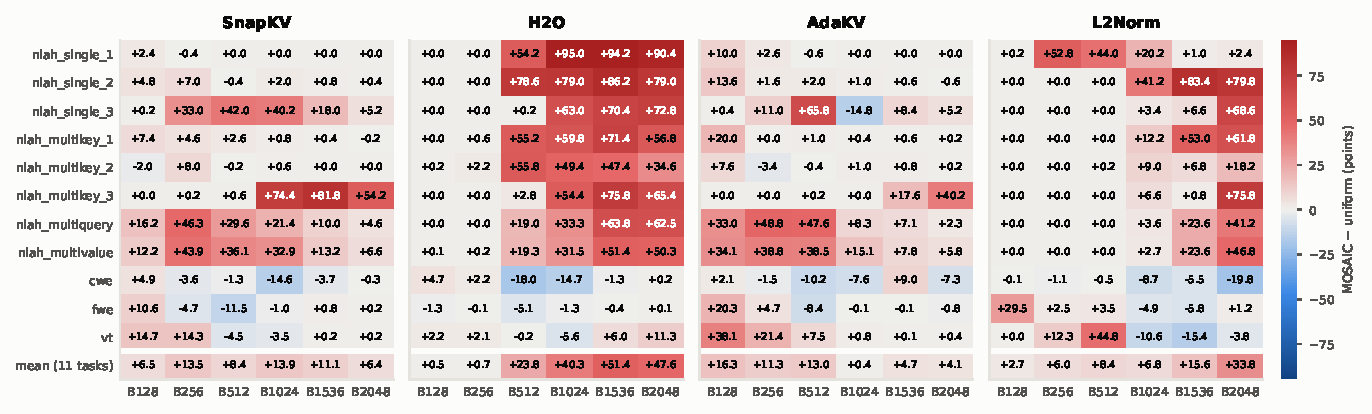
\includegraphics[width=\textwidth]{figures/figure_heat_ruler_mistral.pdf}
  \caption{\textbf{RULER subtask gains of MOSAIC over uniform, Mistral-7B-Instruct-v0.2} (the $\Delta$ rows of Table~\ref{tab:app-ruler-mistral}, points), drawn as Figure~\ref{fig:app-heat-ruler}.}
  \label{fig:app-heat-ruler-mistral}
\end{figure*}

\begin{table*}[tp]
  \centering
  \scriptsize
  \setlength{\tabcolsep}{4pt}
  \renewcommand{\arraystretch}{0.92}
  \begin{tabular}{@{} c l rrrrrrrrrrrrr @{}}
    \toprule
    \textbf{Budget} & & \textbf{S1} & \textbf{S2} & \textbf{S3} & \textbf{MK1} & \textbf{MK2} & \textbf{MK3} & \textbf{MQ} & \textbf{MV} & \textbf{CWE} & \textbf{FWE} & \textbf{VT} & \textbf{NIAH} & \textbf{All} \\
    \midrule
    \multicolumn{15}{c}{\textbf{SnapKV}} \\
    \midrule
    \multirow{2}{*}{128} & Uniform & 96.8 & 83.0 & 0.0 & 80.4 & \textbf{69.0} & 0.0 & 4.7 & 5.2 & 8.8 & 61.3 & 40.6 & 42.4 & 40.9 \\
     & MOSAIC & \textbf{99.2} & \textbf{87.8} & \textbf{0.2} & \textbf{87.8} & 67.0 & 0.0 & \textbf{20.9} & \textbf{17.4} & \textbf{13.8} & \textbf{71.9} & \textbf{55.3} & \textbf{47.5} & \textbf{47.4} \\
    \cmidrule(l){1-15}
    \multirow{2}{*}{256} & Uniform & \textbf{100.0} & 90.4 & 1.4 & 90.6 & 86.6 & 0.0 & 14.8 & 12.9 & \textbf{24.1} & \textbf{78.9} & 69.3 & 49.6 & 51.7 \\
     & MOSAIC & 99.6 & \textbf{97.4} & \textbf{34.4} & \textbf{95.2} & \textbf{94.6} & \textbf{0.2} & \textbf{61.1} & \textbf{56.9} & 20.5 & 74.1 & \textbf{83.6} & \textbf{67.4} & \textbf{65.2} \\
    \cmidrule(l){1-15}
    \multirow{2}{*}{512} & Uniform & 100.0 & \textbf{95.4} & 16.8 & 94.2 & \textbf{94.4} & 0.0 & 38.9 & 25.6 & \textbf{50.3} & \textbf{85.8} & \textbf{89.7} & 58.2 & 62.8 \\
     & MOSAIC & 100.0 & 95.0 & \textbf{58.8} & \textbf{96.8} & 94.2 & \textbf{0.6} & \textbf{68.5} & \textbf{61.8} & 48.9 & 74.3 & 85.2 & \textbf{72.0} & \textbf{71.3} \\
    \cmidrule(l){1-15}
    \multirow{2}{*}{1024} & Uniform & 100.0 & 97.8 & 57.0 & 97.0 & 99.2 & 0.0 & 74.9 & 58.4 & \textbf{77.6} & \textbf{89.5} & \textbf{97.0} & 73.0 & 77.1 \\
     & MOSAIC & 100.0 & \textbf{99.8} & \textbf{97.2} & \textbf{97.8} & \textbf{99.8} & \textbf{74.4} & \textbf{96.3} & \textbf{91.2} & 63.0 & 88.5 & 93.6 & \textbf{94.6} & \textbf{91.1} \\
    \cmidrule(l){1-15}
    \multirow{2}{*}{1536} & Uniform & 100.0 & 99.0 & 82.0 & 97.2 & 99.6 & 8.8 & 88.5 & 80.8 & \textbf{86.7} & 90.3 & 98.2 & 82.0 & 84.7 \\
     & MOSAIC & 100.0 & \textbf{99.8} & \textbf{100.0} & \textbf{97.6} & 99.6 & \textbf{90.6} & \textbf{98.5} & \textbf{94.1} & 83.0 & \textbf{91.1} & \textbf{98.5} & \textbf{97.5} & \textbf{95.7} \\
    \cmidrule(l){1-15}
    \multirow{2}{*}{2048} & Uniform & 100.0 & 99.4 & 92.4 & \textbf{97.6} & 99.8 & 37.4 & 94.3 & 90.5 & \textbf{91.1} & 91.1 & 98.9 & 88.9 & 90.2 \\
     & MOSAIC & 100.0 & \textbf{99.8} & \textbf{97.6} & 97.4 & 99.8 & \textbf{91.6} & \textbf{98.9} & \textbf{97.1} & 90.7 & \textbf{91.3} & \textbf{99.0} & \textbf{97.8} & \textbf{96.7} \\
    \midrule
    \multicolumn{15}{c}{\textbf{H2O}} \\
    \midrule
    \multirow{2}{*}{128} & Uniform & 0.0 & 0.0 & 0.0 & 0.0 & 1.0 & 0.0 & 0.0 & 0.0 & 26.9 & \textbf{76.5} & 7.2 & 0.1 & 10.1 \\
     & MOSAIC & 0.0 & 0.0 & 0.0 & 0.0 & \textbf{1.2} & 0.0 & 0.0 & \textbf{0.1} & \textbf{31.6} & 75.1 & \textbf{9.4} & \textbf{0.2} & \textbf{10.7} \\
    \cmidrule(l){1-15}
    \multirow{2}{*}{256} & Uniform & 0.0 & 0.0 & 0.0 & 0.2 & 3.4 & 0.0 & 0.1 & 0.1 & 55.0 & 83.9 & 12.3 & 0.5 & 14.1 \\
     & MOSAIC & 0.0 & 0.0 & 0.0 & \textbf{0.8} & \textbf{5.6} & 0.0 & 0.1 & \textbf{0.3} & \textbf{57.2} & 83.9 & \textbf{14.4} & \textbf{0.8} & \textbf{14.8} \\
    \cmidrule(l){1-15}
    \multirow{2}{*}{512} & Uniform & 0.4 & 0.4 & 0.0 & 3.0 & 11.0 & 0.2 & 0.6 & 0.8 & \textbf{75.2} & \textbf{90.5} & \textbf{29.2} & 2.1 & 19.2 \\
     & MOSAIC & \textbf{54.6} & \textbf{79.0} & \textbf{0.2} & \textbf{58.2} & \textbf{66.8} & \textbf{3.0} & \textbf{19.6} & \textbf{20.2} & 57.1 & 85.4 & 28.9 & \textbf{37.7} & \textbf{43.0} \\
    \cmidrule(l){1-15}
    \multirow{2}{*}{1024} & Uniform & 2.8 & 2.0 & 0.0 & 9.8 & 27.8 & 3.4 & 4.5 & 6.7 & \textbf{88.4} & \textbf{92.1} & \textbf{67.0} & 7.1 & 27.7 \\
     & MOSAIC & \textbf{97.8} & \textbf{81.0} & \textbf{63.0} & \textbf{69.6} & \textbf{77.2} & \textbf{57.8} & \textbf{37.8} & \textbf{38.1} & 73.7 & 90.9 & 61.4 & \textbf{65.3} & \textbf{68.0} \\
    \cmidrule(l){1-15}
    \multirow{2}{*}{1536} & Uniform & 3.8 & 7.8 & 0.0 & 17.4 & 41.6 & 12.6 & 10.9 & 14.6 & \textbf{92.1} & \textbf{92.7} & 80.0 & 13.6 & 34.0 \\
     & MOSAIC & \textbf{98.0} & \textbf{94.0} & \textbf{70.4} & \textbf{88.8} & \textbf{89.0} & \textbf{88.4} & \textbf{74.8} & \textbf{66.0} & 90.8 & 92.3 & \textbf{86.0} & \textbf{83.7} & \textbf{85.3} \\
    \cmidrule(l){1-15}
    \multirow{2}{*}{2048} & Uniform & 9.6 & 19.4 & 0.0 & 28.0 & 54.0 & 27.4 & 18.8 & 23.4 & 93.7 & 92.9 & 84.4 & 22.6 & 41.1 \\
     & MOSAIC & \textbf{100.0} & \textbf{98.4} & \textbf{72.8} & \textbf{84.8} & \textbf{88.6} & \textbf{92.8} & \textbf{81.2} & \textbf{73.7} & \textbf{94.0} & \textbf{93.0} & \textbf{95.7} & \textbf{86.5} & \textbf{88.6} \\
    \midrule
    \multicolumn{15}{c}{\textbf{AdaKV}} \\
    \midrule
    \multirow{2}{*}{128} & Uniform & 79.8 & 77.2 & 0.0 & 70.8 & 77.2 & 0.0 & 2.4 & 4.2 & 11.4 & 45.4 & 31.3 & 38.9 & 36.3 \\
     & MOSAIC & \textbf{89.8} & \textbf{90.8} & \textbf{0.4} & \textbf{90.8} & \textbf{84.8} & 0.0 & \textbf{35.4} & \textbf{38.2} & \textbf{13.5} & \textbf{65.7} & \textbf{69.4} & \textbf{53.8} & \textbf{52.6} \\
    \cmidrule(l){1-15}
    \multirow{2}{*}{256} & Uniform & 97.2 & 90.4 & 0.4 & 91.0 & \textbf{91.0} & 0.0 & 8.5 & 12.2 & \textbf{19.2} & 76.5 & 52.8 & 48.8 & 49.0 \\
     & MOSAIC & \textbf{99.8} & \textbf{92.0} & \textbf{11.4} & 91.0 & 87.6 & 0.0 & \textbf{57.2} & \textbf{51.0} & 17.8 & \textbf{81.1} & \textbf{74.2} & \textbf{61.3} & \textbf{60.3} \\
    \cmidrule(l){1-15}
    \multirow{2}{*}{512} & Uniform & \textbf{100.0} & 95.2 & 14.2 & 95.2 & \textbf{95.6} & 0.0 & 35.5 & 32.2 & \textbf{35.3} & \textbf{85.9} & 81.1 & 58.5 & 60.9 \\
     & MOSAIC & 99.4 & \textbf{97.2} & \textbf{80.0} & \textbf{96.2} & 95.2 & \textbf{0.2} & \textbf{83.1} & \textbf{70.8} & 25.1 & 77.5 & \textbf{88.6} & \textbf{77.8} & \textbf{73.9} \\
    \cmidrule(l){1-15}
    \multirow{2}{*}{1024} & Uniform & 100.0 & 98.0 & \textbf{63.4} & 97.0 & 97.6 & 0.0 & 76.0 & 65.8 & \textbf{62.0} & \textbf{88.2} & 95.7 & 74.7 & 76.7 \\
     & MOSAIC & 100.0 & \textbf{99.0} & 48.6 & \textbf{97.4} & \textbf{98.6} & 0.0 & \textbf{84.2} & \textbf{80.9} & 54.5 & 88.1 & \textbf{96.6} & \textbf{76.1} & \textbf{77.1} \\
    \cmidrule(l){1-15}
    \multirow{2}{*}{1536} & Uniform & 100.0 & 99.0 & 84.2 & 97.2 & 98.8 & 1.4 & 89.0 & 83.0 & 79.6 & 89.7 & 97.6 & 81.6 & 83.6 \\
     & MOSAIC & 100.0 & \textbf{99.6} & \textbf{92.6} & \textbf{97.8} & \textbf{99.6} & \textbf{19.0} & \textbf{96.2} & \textbf{90.8} & \textbf{88.6} & 89.7 & \textbf{97.7} & \textbf{86.9} & \textbf{88.3} \\
    \cmidrule(l){1-15}
    \multirow{2}{*}{2048} & Uniform & 100.0 & \textbf{99.6} & 92.8 & 97.6 & 99.4 & 13.0 & 94.1 & 90.7 & \textbf{86.9} & \textbf{90.7} & 98.5 & 85.9 & 87.6 \\
     & MOSAIC & 100.0 & 99.0 & \textbf{98.0} & \textbf{97.8} & \textbf{99.6} & \textbf{53.2} & \textbf{96.4} & \textbf{96.5} & 79.6 & 89.9 & \textbf{98.9} & \textbf{92.6} & \textbf{91.7} \\
    \midrule
    \multicolumn{15}{c}{\textbf{L2Norm}} \\
    \midrule
    \multirow{2}{*}{128} & Uniform & 0.0 & 0.0 & 0.0 & 0.0 & 0.0 & 0.0 & 0.0 & 0.0 & \textbf{0.3} & 6.7 & 0.0 & 0.0 & 0.6 \\
     & MOSAIC & \textbf{0.2} & 0.0 & 0.0 & 0.0 & 0.0 & 0.0 & 0.0 & 0.0 & 0.2 & \textbf{36.1} & 0.0 & 0.0 & \textbf{3.3} \\
    \cmidrule(l){1-15}
    \multirow{2}{*}{256} & Uniform & 0.2 & 0.0 & 0.0 & 0.0 & 0.0 & 0.0 & 0.0 & 0.0 & \textbf{1.5} & 44.9 & 0.0 & 0.0 & 4.2 \\
     & MOSAIC & \textbf{53.0} & 0.0 & 0.0 & 0.0 & 0.0 & 0.0 & 0.0 & 0.0 & 0.5 & \textbf{47.4} & \textbf{12.4} & \textbf{6.6} & \textbf{10.3} \\
    \cmidrule(l){1-15}
    \multirow{2}{*}{512} & Uniform & 41.0 & 0.0 & 0.0 & 0.0 & 0.0 & 0.0 & 0.0 & 0.0 & \textbf{7.2} & 65.8 & 7.6 & 5.1 & 11.1 \\
     & MOSAIC & \textbf{85.0} & 0.0 & 0.0 & 0.0 & \textbf{0.2} & 0.0 & 0.0 & 0.0 & 6.7 & \textbf{69.3} & \textbf{52.4} & \textbf{10.7} & \textbf{19.4} \\
    \cmidrule(l){1-15}
    \multirow{2}{*}{1024} & Uniform & 79.8 & 0.0 & 0.0 & 0.0 & 0.0 & 0.0 & 0.0 & 0.0 & \textbf{18.1} & \textbf{77.5} & \textbf{76.0} & 10.0 & 22.9 \\
     & MOSAIC & \textbf{100.0} & \textbf{41.2} & \textbf{3.4} & \textbf{12.2} & \textbf{9.0} & \textbf{6.6} & \textbf{3.6} & \textbf{2.7} & 9.5 & 72.5 & 65.5 & \textbf{22.3} & \textbf{29.7} \\
    \cmidrule(l){1-15}
    \multirow{2}{*}{1536} & Uniform & 94.4 & 0.6 & 0.0 & 0.2 & 0.8 & 0.0 & 0.0 & 0.0 & \textbf{32.7} & \textbf{83.1} & \textbf{91.7} & 12.0 & 27.6 \\
     & MOSAIC & \textbf{95.4} & \textbf{84.0} & \textbf{6.6} & \textbf{53.2} & \textbf{7.6} & \textbf{0.8} & \textbf{23.6} & \textbf{23.6} & 27.1 & 77.3 & 76.3 & \textbf{36.9} & \textbf{43.2} \\
    \cmidrule(l){1-15}
    \multirow{2}{*}{2048} & Uniform & 97.6 & 0.8 & 0.0 & 0.0 & 2.0 & 1.0 & 0.0 & 0.0 & \textbf{54.8} & 85.9 & \textbf{96.0} & 12.7 & 30.7 \\
     & MOSAIC & \textbf{100.0} & \textbf{80.6} & \textbf{68.6} & \textbf{61.8} & \textbf{20.2} & \textbf{76.8} & \textbf{41.2} & \textbf{46.8} & 35.0 & \textbf{87.1} & 92.2 & \textbf{62.0} & \textbf{64.6} \\
    \bottomrule
  \end{tabular}
  \caption{\textbf{RULER subtask accuracy (string match, \%), uniform vs.\ MOSAIC per cell, Mistral-7B-Instruct-v0.2.}}
  \label{tab:app-ruler-mistral}
\end{table*}


\subsection{LongBench Dataset Breakdown}
\label{app:dataset-reg}

LongBench scores are category means over two or three datasets. Tables~\ref{tab:app-lb} (Llama-3-8B-Instruct) and~\ref{tab:app-lb-mistral} (Mistral-7B-Instruct-v0.2) break each LongBench cell into its datasets, comparing uniform with MOSAIC's final configuration (the better of Winner and NAS-refined on the category mean); Figures~\ref{fig:app-heat-lb} and~\ref{fig:app-heat-lb-mistral} show the per-dataset gains as heatmaps. On Llama, the final configuration falls below uniform on at least one dataset in 23 of 60 cells, and in 19 of them the category mean is still above uniform; on Mistral this happens in 12 of 52 cells.

\begin{figure*}[tp]
  \centering
  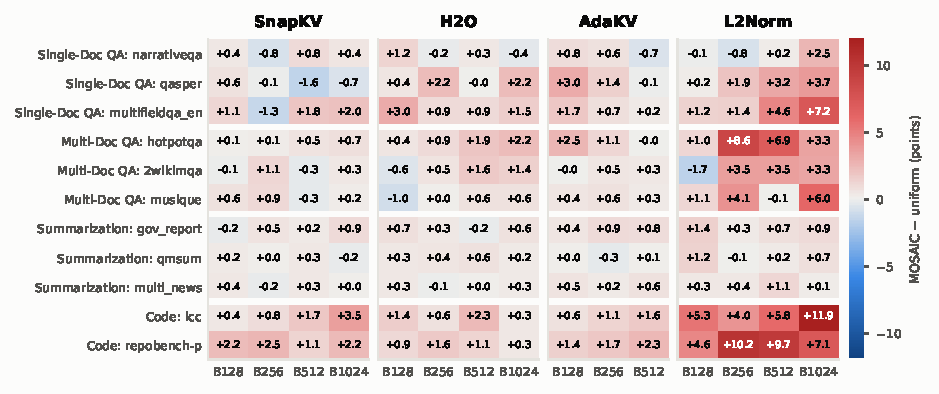
\includegraphics[width=\textwidth]{figures/figure_heat_lb.pdf}
  \caption{\textbf{LongBench dataset gains of MOSAIC over uniform, Llama-3-8B-Instruct} (full data, points; the uniform and MOSAIC rows of Table~\ref{tab:app-lb}). Rows: datasets grouped by category; columns: budget; grey: no cell. Red: MOSAIC above uniform; blue: below.}
  \label{fig:app-heat-lb}
\end{figure*}

\begin{figure*}[tp]
  \centering
  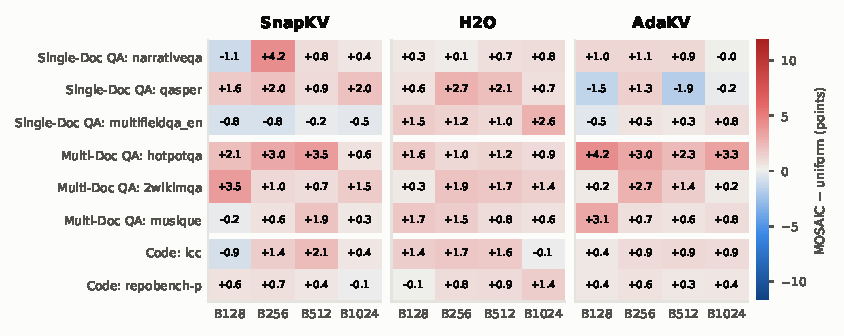
\includegraphics[width=0.899\textwidth]{figures/figure_heat_lb_mistral.pdf}

  \vspace{6pt}
  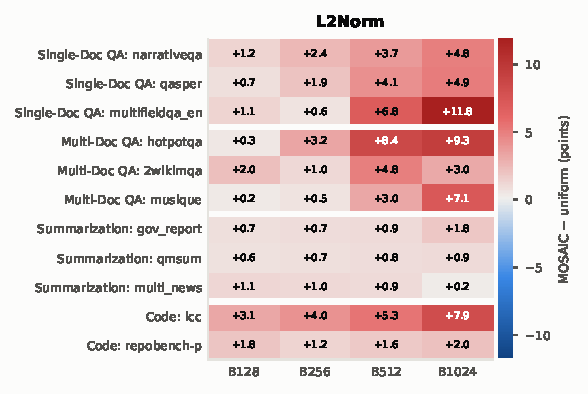
\includegraphics[width=0.627\textwidth]{figures/figure_heat_lb_mistral_l2.pdf}
  \caption{\textbf{LongBench dataset gains of MOSAIC over uniform, Mistral-7B-Instruct-v0.2} (full data, points; the uniform and MOSAIC rows of Table~\ref{tab:app-lb-mistral}), drawn as Figure~\ref{fig:app-heat-lb}; both panels share one colour scale. Top: SnapKV, H2O and AdaKV, which have no Summarization cells; bottom: L2Norm, all four tasks.}
  \label{fig:app-heat-lb-mistral}
\end{figure*}

\begin{table*}[tp]
  \centering
  \scriptsize
  \setlength{\tabcolsep}{3pt}
  \renewcommand{\arraystretch}{0.92}
  \begin{tabular}{@{} c l rrrr rrrr rrrr rrr @{}}
    \toprule
    & & \multicolumn{4}{c}{\textbf{Single-Doc QA}} & \multicolumn{4}{c}{\textbf{Multi-Doc QA}} & \multicolumn{4}{c}{\textbf{Summarization}} & \multicolumn{3}{c}{\textbf{Code}} \\
    \cmidrule(lr){3-6} \cmidrule(lr){7-10} \cmidrule(lr){11-14} \cmidrule(lr){15-17}
    \textbf{Budget} & & NQA & Qasper & MFQA & Mean & HQA & 2Wiki & MuSiQue & Mean & GovRep & QMSum & MNews & Mean & LCC & RepoB-P & Mean \\
    \midrule
    \multicolumn{17}{c}{\textbf{SnapKV}} \\
    \midrule
    \multirow{2}{*}{128} & Uniform & 18.70 & 35.14 & 45.08 & 32.97 & 45.94 & \textbf{36.39} & 22.13 & 34.82 & \textbf{21.01} & 20.35 & 21.73 & 21.03 & 56.90 & 52.73 & 54.81 \\
     & MOSAIC & \textbf{19.07} & \textbf{35.76} & \textbf{46.18} & \textbf{33.67} & \textbf{46.02} & 36.28 & \textbf{22.77} & \textbf{35.02} & 20.82 & \textbf{20.54} & \textbf{22.09} & \textbf{21.15} & \textbf{57.25} & \textbf{54.94} & \textbf{56.09} \\
    \cmidrule(l){1-17}
    \multirow{2}{*}{256} & Uniform & \textbf{19.96} & \textbf{39.44} & \textbf{46.35} & \textbf{35.25} & 46.94 & 37.50 & 22.36 & 35.60 & 22.25 & 21.09 & \textbf{23.57} & 22.30 & 58.23 & 53.12 & 55.67 \\
     & MOSAIC & 19.21 & 39.32 & 45.01 & 34.51 & \textbf{47.05} & \textbf{38.58} & \textbf{23.30} & \textbf{36.31} & \textbf{22.77} & 21.09 & 23.37 & \textbf{22.41} & \textbf{59.05} & \textbf{55.61} & \textbf{57.33} \\
    \cmidrule(l){1-17}
    \multirow{2}{*}{512} & Uniform & 19.99 & \textbf{41.86} & 46.06 & 35.97 & 46.72 & \textbf{37.98} & \textbf{22.60} & \textbf{35.77} & 24.06 & 21.37 & 24.88 & 23.44 & 59.16 & 54.31 & 56.73 \\
     & MOSAIC & \textbf{20.83} & 40.29 & \textbf{47.86} & \textbf{36.33} & \textbf{47.20} & 37.69 & 22.29 & 35.73 & \textbf{24.26} & \textbf{21.69} & \textbf{25.17} & \textbf{23.71} & \textbf{60.89} & \textbf{55.44} & \textbf{58.16} \\
    \cmidrule(l){1-17}
    \multirow{2}{*}{1024} & Uniform & 20.66 & \textbf{42.64} & 46.02 & 36.44 & 47.18 & 38.40 & 22.02 & 35.87 & 25.56 & \textbf{22.31} & 26.67 & 24.85 & 58.35 & 53.69 & 56.02 \\
     & MOSAIC & \textbf{21.07} & 41.90 & \textbf{48.05} & \textbf{37.01} & \textbf{47.86} & \textbf{38.73} & \textbf{22.19} & \textbf{36.26} & \textbf{26.49} & 22.12 & \textbf{26.70} & \textbf{25.10} & \textbf{61.89} & \textbf{55.93} & \textbf{58.91} \\
    \midrule
    \multicolumn{17}{c}{\textbf{H2O}} \\
    \midrule
    \multirow{2}{*}{128} & Uniform & 17.70 & 31.10 & 35.84 & 28.21 & 43.42 & \textbf{33.38} & \textbf{20.91} & \textbf{32.57} & 23.02 & 17.79 & 24.82 & 21.88 & 49.92 & 42.00 & 45.96 \\
     & MOSAIC & \textbf{18.86} & \textbf{31.49} & \textbf{38.82} & \textbf{29.72} & \textbf{43.80} & 32.78 & 19.91 & 32.16 & \textbf{23.72} & \textbf{18.10} & \textbf{25.12} & \textbf{22.31} & \textbf{51.33} & \textbf{42.94} & \textbf{47.13} \\
    \cmidrule(l){1-17}
    \multirow{2}{*}{256} & Uniform & \textbf{18.66} & 32.31 & 38.91 & 29.96 & 44.03 & 33.42 & 19.90 & 32.45 & 24.78 & 18.94 & \textbf{25.68} & 23.13 & 53.45 & 45.54 & 49.50 \\
     & MOSAIC & 18.44 & \textbf{34.49} & \textbf{39.84} & \textbf{30.92} & \textbf{44.88} & \textbf{33.94} & \textbf{19.94} & \textbf{32.92} & \textbf{25.12} & \textbf{19.32} & 25.56 & \textbf{23.33} & \textbf{54.04} & \textbf{47.14} & \textbf{50.59} \\
    \cmidrule(l){1-17}
    \multirow{2}{*}{512} & Uniform & 19.20 & \textbf{35.71} & 42.32 & 32.41 & 43.90 & 34.29 & 20.75 & 32.98 & \textbf{26.95} & 19.43 & 26.28 & 24.22 & 55.97 & 49.65 & 52.81 \\
     & MOSAIC & \textbf{19.49} & 35.70 & \textbf{43.21} & \textbf{32.80} & \textbf{45.75} & \textbf{35.92} & \textbf{21.32} & \textbf{34.33} & 26.72 & \textbf{20.03} & \textbf{26.30} & \textbf{24.35} & \textbf{58.23} & \textbf{50.78} & \textbf{54.50} \\
    \cmidrule(l){1-17}
    \multirow{2}{*}{1024} & Uniform & \textbf{19.26} & 38.36 & 43.19 & 33.60 & 44.33 & 35.56 & 20.72 & 33.54 & 27.94 & 20.05 & 26.93 & 24.97 & 59.62 & 54.23 & 56.92 \\
     & MOSAIC & 18.82 & \textbf{40.58} & \textbf{44.68} & \textbf{34.69} & \textbf{46.54} & \textbf{36.94} & \textbf{21.30} & \textbf{34.93} & \textbf{28.52} & \textbf{20.24} & \textbf{27.19} & \textbf{25.32} & \textbf{59.92} & \textbf{54.54} & \textbf{57.23} \\
    \midrule
    \multicolumn{17}{c}{\textbf{AdaKV}} \\
    \midrule
    \multirow{2}{*}{128} & Uniform & 18.60 & 34.52 & 45.36 & 32.83 & 45.50 & \textbf{36.81} & 22.67 & 34.99 & 21.57 & 21.26 & 22.32 & 21.72 & 59.83 & 54.77 & 57.30 \\
     & MOSAIC & \textbf{19.39} & \textbf{37.49} & \textbf{47.05} & \textbf{34.64} & \textbf{47.98} & 36.80 & \textbf{23.10} & \textbf{35.96} & \textbf{22.02} & \textbf{21.28} & \textbf{22.86} & \textbf{22.05} & \textbf{60.44} & \textbf{56.13} & \textbf{58.28} \\
    \cmidrule(l){1-17}
    \multirow{2}{*}{256} & Uniform & 20.09 & 39.10 & 46.04 & 35.08 & 46.07 & 37.57 & 22.63 & 35.42 & 22.57 & \textbf{21.81} & 23.77 & 22.72 & 60.02 & 56.36 & 58.19 \\
     & MOSAIC & \textbf{20.69} & \textbf{40.46} & \textbf{46.78} & \textbf{35.98} & \textbf{47.18} & \textbf{38.03} & \textbf{23.21} & \textbf{36.14} & \textbf{23.48} & 21.53 & \textbf{23.99} & \textbf{23.00} & \textbf{61.17} & \textbf{58.08} & \textbf{59.62} \\
    \cmidrule(l){1-17}
    \multirow{2}{*}{512} & Uniform & \textbf{21.32} & \textbf{41.86} & 46.87 & \textbf{36.68} & \textbf{47.20} & 38.68 & 22.53 & 36.14 & 23.88 & 21.86 & 25.12 & 23.62 & 61.09 & 56.31 & 58.70 \\
     & MOSAIC & 20.65 & 41.74 & \textbf{47.07} & 36.49 & 47.19 & \textbf{39.00} & \textbf{22.79} & \textbf{36.33} & \textbf{24.63} & \textbf{21.94} & \textbf{25.68} & \textbf{24.08} & \textbf{62.71} & \textbf{58.65} & \textbf{60.68} \\
    \midrule
    \multicolumn{17}{c}{\textbf{L2Norm}} \\
    \midrule
    \multirow{2}{*}{128} & Uniform & \textbf{5.15} & 15.36 & 10.10 & 10.20 & 11.70 & \textbf{10.32} & 5.24 & 9.09 & 17.95 & 15.50 & 19.73 & 17.73 & 23.23 & 21.85 & 22.54 \\
     & MOSAIC & 5.02 & \textbf{15.53} & \textbf{11.34} & \textbf{10.63} & \textbf{12.73} & 8.66 & \textbf{6.31} & \textbf{9.23} & \textbf{19.32} & \textbf{16.72} & \textbf{20.02} & \textbf{18.69} & \textbf{28.55} & \textbf{26.41} & \textbf{27.48} \\
    \cmidrule(l){1-17}
    \multirow{2}{*}{256} & Uniform & \textbf{9.01} & 18.58 & 14.15 & 13.91 & 18.39 & 13.17 & 8.13 & 13.23 & 19.85 & \textbf{17.55} & 21.97 & 19.79 & 27.00 & 20.15 & 23.57 \\
     & MOSAIC & 8.24 & \textbf{20.50} & \textbf{15.54} & \textbf{14.76} & \textbf{27.00} & \textbf{16.69} & \textbf{12.22} & \textbf{18.64} & \textbf{20.11} & 17.49 & \textbf{22.33} & \textbf{19.98} & \textbf{30.99} & \textbf{30.39} & \textbf{30.69} \\
    \cmidrule(l){1-17}
    \multirow{2}{*}{512} & Uniform & 12.47 & 22.02 & 20.95 & 18.48 & 31.48 & 19.41 & \textbf{15.30} & 22.06 & 21.40 & 18.77 & 23.73 & 21.30 & 31.33 & 24.96 & 28.14 \\
     & MOSAIC & \textbf{12.65} & \textbf{25.18} & \textbf{25.57} & \textbf{21.13} & \textbf{38.34} & \textbf{22.91} & 15.22 & \textbf{25.49} & \textbf{22.09} & \textbf{18.96} & \textbf{24.79} & \textbf{21.95} & \textbf{37.15} & \textbf{34.65} & \textbf{35.90} \\
    \cmidrule(l){1-17}
    \multirow{2}{*}{1024} & Uniform & 16.19 & 29.28 & 28.78 & 24.75 & 40.64 & 29.42 & 16.09 & 28.72 & 22.91 & 19.98 & 26.14 & 23.01 & 37.05 & 32.85 & 34.95 \\
     & MOSAIC & \textbf{18.67} & \textbf{32.94} & \textbf{36.01} & \textbf{29.21} & \textbf{43.95} & \textbf{32.68} & \textbf{22.08} & \textbf{32.90} & \textbf{23.80} & \textbf{20.64} & \textbf{26.28} & \textbf{23.57} & \textbf{48.99} & \textbf{39.95} & \textbf{44.47} \\
    \bottomrule
  \end{tabular}
  \caption{\textbf{LongBench dataset scores, uniform vs.\ MOSAIC per cell, Llama-3-8B-Instruct} (full data); bold: the better of the two in each column. NQA: NarrativeQA; MFQA: MultiFieldQA-en; HQA: HotpotQA; 2Wiki: 2WikiMQA; GovRep: GovReport; MNews: Multi-News; RepoB-P: RepoBench-P.}
  \label{tab:app-lb}
\end{table*}

\begin{table*}[tp]
  \centering
  \scriptsize
  \setlength{\tabcolsep}{3pt}
  \renewcommand{\arraystretch}{0.92}
  \begin{tabular}{@{} c l rrrr rrrr rrr @{}}
    \toprule
    & & \multicolumn{4}{c}{\textbf{Single-Doc QA}} & \multicolumn{4}{c}{\textbf{Multi-Doc QA}} & \multicolumn{3}{c}{\textbf{Code}} \\
    \cmidrule(lr){3-6} \cmidrule(lr){7-10} \cmidrule(lr){11-13}
    \textbf{Budget} & & NQA & Qasper & MFQA & Mean & HQA & 2Wiki & MuSiQue & Mean & LCC & RepoB-P & Mean \\
    \midrule
    \multicolumn{13}{c}{\textbf{SnapKV}} \\
    \midrule
    \multirow{2}{*}{128} & Uniform & \textbf{21.54} & 21.91 & \textbf{45.38} & \textbf{29.61} & 33.94 & 22.04 & \textbf{15.61} & 23.86 & \textbf{52.20} & 47.31 & \textbf{49.76} \\
     & MOSAIC & 20.39 & \textbf{23.49} & 44.61 & 29.50 & \textbf{36.03} & \textbf{25.58} & 15.42 & \textbf{25.68} & 51.33 & \textbf{47.90} & 49.61 \\
    \cmidrule(l){1-13}
    \multirow{2}{*}{256} & Uniform & 22.03 & 24.99 & \textbf{48.20} & 31.74 & 36.62 & 25.11 & 15.14 & 25.62 & 53.88 & 50.30 & 52.09 \\
     & MOSAIC & \textbf{26.26} & \textbf{26.94} & 47.39 & \textbf{33.53} & \textbf{39.63} & \textbf{26.07} & \textbf{15.73} & \textbf{27.14} & \textbf{55.32} & \textbf{50.97} & \textbf{53.14} \\
    \cmidrule(l){1-13}
    \multirow{2}{*}{512} & Uniform & 24.13 & 28.84 & \textbf{48.75} & 33.91 & 38.82 & 25.48 & 15.10 & 26.47 & 55.10 & 52.44 & 53.77 \\
     & MOSAIC & \textbf{24.92} & \textbf{29.69} & 48.55 & \textbf{34.39} & \textbf{42.35} & \textbf{26.22} & \textbf{17.02} & \textbf{28.53} & \textbf{57.23} & \textbf{52.88} & \textbf{55.05} \\
    \cmidrule(l){1-13}
    \multirow{2}{*}{1024} & Uniform & 25.03 & 30.37 & \textbf{49.57} & 34.99 & 41.84 & 26.53 & 18.03 & 28.80 & 56.87 & \textbf{53.60} & 55.23 \\
     & MOSAIC & \textbf{25.40} & \textbf{32.34} & 49.11 & \textbf{35.62} & \textbf{42.45} & \textbf{28.01} & \textbf{18.33} & \textbf{29.60} & \textbf{57.30} & 53.46 & \textbf{55.38} \\
    \midrule
    \multicolumn{13}{c}{\textbf{H2O}} \\
    \midrule
    \multirow{2}{*}{128} & Uniform & 22.16 & 20.57 & 35.88 & 26.20 & 30.65 & 19.70 & 12.96 & 21.10 & 42.71 & \textbf{36.47} & 39.59 \\
     & MOSAIC & \textbf{22.48} & \textbf{21.20} & \textbf{37.38} & \textbf{27.02} & \textbf{32.23} & \textbf{19.96} & \textbf{14.67} & \textbf{22.29} & \textbf{44.16} & 36.40 & \textbf{40.28} \\
    \cmidrule(l){1-13}
    \multirow{2}{*}{256} & Uniform & 22.23 & 22.48 & 39.06 & 27.92 & 34.47 & 20.86 & 15.78 & 23.70 & 46.88 & 39.30 & 43.09 \\
     & MOSAIC & \textbf{22.36} & \textbf{25.14} & \textbf{40.26} & \textbf{29.25} & \textbf{35.48} & \textbf{22.77} & \textbf{17.24} & \textbf{25.16} & \textbf{48.59} & \textbf{40.06} & \textbf{44.33} \\
    \cmidrule(l){1-13}
    \multirow{2}{*}{512} & Uniform & 23.47 & 26.40 & 41.70 & 30.52 & 35.29 & 22.41 & 17.84 & 25.18 & 50.81 & 42.05 & 46.43 \\
     & MOSAIC & \textbf{24.17} & \textbf{28.51} & \textbf{42.71} & \textbf{31.80} & \textbf{36.47} & \textbf{24.15} & \textbf{18.67} & \textbf{26.43} & \textbf{52.40} & \textbf{42.96} & \textbf{47.68} \\
    \cmidrule(l){1-13}
    \multirow{2}{*}{1024} & Uniform & 23.44 & 29.67 & 43.32 & 32.14 & 36.21 & 25.76 & 17.76 & 26.58 & \textbf{54.07} & 45.23 & 49.65 \\
     & MOSAIC & \textbf{24.23} & \textbf{30.35} & \textbf{45.93} & \textbf{33.50} & \textbf{37.07} & \textbf{27.12} & \textbf{18.38} & \textbf{27.52} & 53.97 & \textbf{46.64} & \textbf{50.30} \\
    \midrule
    \multicolumn{13}{c}{\textbf{AdaKV}} \\
    \midrule
    \multirow{2}{*}{128} & Uniform & 21.59 & \textbf{24.37} & \textbf{46.76} & \textbf{30.91} & 35.63 & 25.63 & 14.56 & 25.27 & 53.19 & 48.96 & 51.08 \\
     & MOSAIC & \textbf{22.63} & 22.84 & 46.25 & 30.57 & \textbf{39.82} & \textbf{25.86} & \textbf{17.66} & \textbf{27.78} & \textbf{53.54} & \textbf{49.31} & \textbf{51.42} \\
    \cmidrule(l){1-13}
    \multirow{2}{*}{256} & Uniform & 23.87 & 27.15 & 48.40 & 33.14 & 38.35 & 25.21 & 16.41 & 26.66 & 54.67 & 50.64 & 52.66 \\
     & MOSAIC & \textbf{24.96} & \textbf{28.49} & \textbf{48.92} & \textbf{34.12} & \textbf{41.40} & \textbf{27.87} & \textbf{17.14} & \textbf{28.80} & \textbf{55.57} & \textbf{51.27} & \textbf{53.42} \\
    \cmidrule(l){1-13}
    \multirow{2}{*}{512} & Uniform & 24.17 & \textbf{30.10} & 49.00 & \textbf{34.42} & 39.95 & 25.37 & 17.55 & 27.62 & 56.02 & 53.28 & 54.65 \\
     & MOSAIC & \textbf{25.10} & 28.20 & \textbf{49.34} & 34.21 & \textbf{42.23} & \textbf{26.82} & \textbf{18.10} & \textbf{29.05} & \textbf{56.95} & \textbf{53.58} & \textbf{55.27} \\
    \cmidrule(l){1-13}
    \multirow{2}{*}{1024} & Uniform & \textbf{24.86} & \textbf{31.37} & 48.67 & 34.97 & 41.18 & 27.36 & 18.03 & 28.86 & 56.77 & 53.38 & 55.08 \\
     & MOSAIC & 24.85 & 31.13 & \textbf{49.48} & \textbf{35.15} & \textbf{44.48} & \textbf{27.61} & \textbf{18.79} & \textbf{30.29} & \textbf{57.68} & \textbf{53.83} & \textbf{55.75} \\
    \bottomrule
  \end{tabular}

  \vspace{8pt}
  \scriptsize
  \setlength{\tabcolsep}{3pt}
  \renewcommand{\arraystretch}{0.92}
  \begin{tabular}{@{} c l rrrr rrrr rrrr rrr @{}}
    \toprule
    & & \multicolumn{4}{c}{\textbf{Single-Doc QA}} & \multicolumn{4}{c}{\textbf{Multi-Doc QA}} & \multicolumn{4}{c}{\textbf{Summarization}} & \multicolumn{3}{c}{\textbf{Code}} \\
    \cmidrule(lr){3-6} \cmidrule(lr){7-10} \cmidrule(lr){11-14} \cmidrule(lr){15-17}
    \textbf{Budget} & & NQA & Qasper & MFQA & Mean & HQA & 2Wiki & MuSiQue & Mean & GovRep & QMSum & MNews & Mean & LCC & RepoB-P & Mean \\
    \midrule
    \multicolumn{17}{c}{\textbf{L2Norm}} \\
    \midrule
    \multirow{2}{*}{128} & Uniform & 3.52 & 4.35 & 7.21 & 5.03 & 7.33 & 5.48 & 2.08 & 4.96 & 20.11 & 15.11 & 18.84 & 18.02 & 24.95 & 19.94 & 22.45 \\
     & MOSAIC & \textbf{4.71} & \textbf{5.06} & \textbf{8.35} & \textbf{6.04} & \textbf{7.67} & \textbf{7.53} & \textbf{2.32} & \textbf{5.84} & \textbf{20.83} & \textbf{15.71} & \textbf{19.89} & \textbf{18.81} & \textbf{28.01} & \textbf{21.77} & \textbf{24.89} \\
    \cmidrule(l){1-17}
    \multirow{2}{*}{256} & Uniform & 6.65 & 5.71 & 9.44 & 7.27 & 7.64 & 6.76 & 2.79 & 5.73 & 21.55 & 16.37 & 20.90 & 19.61 & 28.00 & 23.16 & 25.58 \\
     & MOSAIC & \textbf{9.04} & \textbf{7.60} & \textbf{9.99} & \textbf{8.88} & \textbf{10.81} & \textbf{7.77} & \textbf{3.29} & \textbf{7.29} & \textbf{22.29} & \textbf{17.06} & \textbf{21.86} & \textbf{20.40} & \textbf{32.03} & \textbf{24.33} & \textbf{28.18} \\
    \cmidrule(l){1-17}
    \multirow{2}{*}{512} & Uniform & 9.08 & 8.36 & 12.06 & 9.83 & 10.96 & 7.11 & 4.57 & 7.55 & 22.49 & 17.56 & 22.62 & 20.89 & 31.11 & 26.25 & 28.68 \\
     & MOSAIC & \textbf{12.74} & \textbf{12.43} & \textbf{18.82} & \textbf{14.66} & \textbf{19.35} & \textbf{11.91} & \textbf{7.62} & \textbf{12.96} & \textbf{23.34} & \textbf{18.33} & \textbf{23.48} & \textbf{21.72} & \textbf{36.39} & \textbf{27.86} & \textbf{32.12} \\
    \cmidrule(l){1-17}
    \multirow{2}{*}{1024} & Uniform & 13.29 & 14.83 & 20.70 & 16.27 & 16.41 & 10.62 & 6.00 & 11.01 & 23.48 & 19.17 & 24.79 & 22.48 & 36.59 & 29.84 & 33.22 \\
     & MOSAIC & \textbf{18.11} & \textbf{19.76} & \textbf{32.51} & \textbf{23.46} & \textbf{25.67} & \textbf{13.58} & \textbf{13.10} & \textbf{17.45} & \textbf{25.23} & \textbf{20.04} & \textbf{24.95} & \textbf{23.41} & \textbf{44.53} & \textbf{31.83} & \textbf{38.18} \\
    \bottomrule
  \end{tabular}
  \caption{\textbf{LongBench dataset scores, uniform vs.\ MOSAIC per cell, Mistral-7B-Instruct-v0.2} (full data); bold: the better of the two in each column. NQA: NarrativeQA; MFQA: MultiFieldQA-en; HQA: HotpotQA; 2Wiki: 2WikiMQA; GovRep: GovReport; MNews: Multi-News; RepoB-P: RepoBench-P. SnapKV, H2O and AdaKV (top) have no Summarization cells; L2Norm (bottom) covers all four tasks.}
  \label{tab:app-lb-mistral}
\end{table*}


\end{document}
